%======================================================================
\chapter{Requirement Analysis}
%======================================================================

% %----------------------------------------------------------------------
% \section{Stakeholder Analysis}
% %----------------------------------------------------------------------

% The successful implementation of the BorBann platform requires a understanding of all parties who may influence or be affected by the system. This stakeholder analysis identifies key individuals and groups, their interests, influence levels, and specific requirements.

%----------------------------------------------------------------------
\section{Stakeholder Analysis}
%----------------------------------------------------------------------

The stakeholder landscape for BorBann includes primary stakeholders who directly interact with the platform and secondary stakeholders who indirectly influence its adoption and effectiveness. Recognizing these groups' specific needs helps develop a platform that delivers value across the real estate ecosystem.

\begin{table}[htbp]
	\centering
	\renewcommand{\arraystretch}{1.3}
	\resizebox{0.95\textwidth}{!}{
		\begin{tabular}{>{\raggedright\arraybackslash}p{0.2\textwidth}>{\raggedright\arraybackslash}p{0.2\textwidth}>{\raggedright\arraybackslash}p{0.3\textwidth}>{\raggedright\arraybackslash}p{0.3\textwidth}}
			\toprule \rowcolor[gray]{0.9}
			\textbf{Stakeholder Category}                        & \textbf{Stakeholder Group} & \textbf{Key Interests}                                                  & \textbf{Primary Requirements}                                                       \\
			\midrule
			\textbf{Primary}                                     & Real Estate Investors      & Environment risk assessment                                             & Advanced analytics, predictive modeling, risk scoring                               \\
			\addlinespace \rowcolor[gray]{0.95} \textbf{Primary} & Homebuyers                 & Affordability, area quality, lifestyle alignment, environmental factors & User-friendly interface, neighborhood insights, price comparisons, risk assessments \\
			\addlinespace \textbf{Secondary}                     & Real Estate Agencies       & Market positioning, client advisement, property valuation               & Property data, reliable market insights                                             \\
			\bottomrule
		\end{tabular}
	}
	\caption{BorBann Platform Stakeholder Summary}
	\label{tab:stakeholder-summary}
\end{table}

The primary stakeholders are direct users who rely on BorBann's capabilities for informed real estate decisions. Their requirements range from investment analytics to intuitive neighborhood quality assessments. Secondary stakeholders like real estate agencies can influence platform adoption and serve as valuable data partners.


\subsection{Primary Stakeholders}

Primary stakeholders are those who directly use or are significantly affected by the BorBann platform. They rely on its capabilities to make informed decisions about real estate investments, purchases, and market trends.

\subsubsection{Real Estate Investors}
Real estate investors use BorBann to identify profitable investment, assess risks, and make data-driven decisions.

\textbf{Interests and Concerns:}
\begin{itemize}
	\item Maximizing return on investment
	\item Identifying growth areas
	\item Risk assessment
	\item Diversification across neighborhoods and property classes
\end{itemize}

\textbf{Requirements:}
\begin{itemize}
	\item Advanced analytics tools that is customizable
	\item Predictive price modeling with easy to understand explaination
	\item Risk scores in each area based on multiple factors
\end{itemize}

\subsubsection{Homebuyers}
Homebuyers rely on BorBann to find properties that align with their budget, lifestyle, and long-term needs. The platform helps them assess affordability, neighborhood quality, and potential risks.

\textbf{Interests and Concerns:}
\begin{itemize}
	\item Property affordability and financing options
	\item Area quality
	\item Location amenities and lifestyle alignment
	\item Environmental factors including flood and pollution risks
	\item Commute time to work, schools, and essential services
	\item School districts and educational quality
\end{itemize}

\textbf{Requirements:}
\begin{itemize}
	\item Intuitive, user-friendly interface with minimal learning curve
	\item Comprehensive neighborhood insights including safety metrics
	\item Price comparison tools with historical context
	\item Property quality and developer reputation metrics
	\item Detailed flood risk and environmental quality assessment
	\item Transit accessibility maps with time-based visualizations
	\item Education quality indicators and school zone mapping
\end{itemize}

\subsection{Secondary Stakeholders}

Secondary stakeholders are indirectly impacted by the BorBann platform, influencing its adoption, data availability, and overall market reach.

\subsubsection{Real Estate Agencies}
Real estate agencies act as intermediaries between property buyers and sellers. They use BorBann to improve their advisory services, gain a competitive edge, and provide market insights to clients.

\textbf{Interests and Concerns:}
\begin{itemize}
	\item Market positioning relative to competitors
	\item Client advisement based on reliable data
	\item Access to comprehensive property information
	\item Accurate property valuation to support transactions
\end{itemize}

\textbf{Influence:}
\begin{itemize}
	\item Potential data partners and platform promoters
	\item Can significantly influence adoption rates among clients
	\item May provide valuable transaction data not available elsewhere
\end{itemize}

%----------------------------------------------------------------------
\section{User Stories}
%----------------------------------------------------------------------

User stories capture the essential needs and goals of the BorBann platform's target users from their perspective. These stories follow the standard format: "As a [user type], I want to [action/feature] so that [benefit/value]."

\begin{longtable}{>{\raggedright\arraybackslash}p{0.4\textwidth}>{\raggedright\arraybackslash}p{0.6\textwidth}}
	\caption{User Stories with Acceptance Criteria\label{tab:user-stories}}\\
	  
	\toprule \rowcolor[gray]{0.9}
	\textbf{User Story} & \textbf{Acceptance Criteria} \\
	\midrule
	\endfirsthead
	  
	\multicolumn{2}{c}{\tablename\ \thetable{} -- Continued from previous page} \\
	\toprule \rowcolor[gray]{0.9}
	\textbf{User Story} & \textbf{Acceptance Criteria} \\
	\midrule
	\endhead
	  
	\midrule
	\multicolumn{2}{r}{Continued on next page} \\
	\endfoot
	  
	\bottomrule
	\endlastfoot
	  
	\multicolumn{2}{l}{\textbf{Customizable Automated Data Integration Pipeline}} \\
	\midrule
	As a non-technical user, I want to input a website URL and have the system automatically generate a scraping configuration, so I can collect data without coding skills &
	\begin{itemize}
	\item System provides visual confirmation of detected data structure
	\item Non-technical users can successfully create a working pipeline in under 5 minutes
	\end{itemize} \\
	  
	\rowcolor[gray]{0.95} 
	As a user, I want to paste multiple URLs from the same website pattern and have the system recognize the common structure, so I can efficiently collect data from similar pages &
	\begin{itemize}
	\item System identifies common patterns across multiple URLs from the same website
	\item A single configuration works for all provided URLs from the same pattern
	\end{itemize} \\
	  
	As a user, I want to upload data files (CSV, JSON) as alternative data sources to integrate with my scraped data &
	\begin{itemize}
	\item System accepts uploads of CSV and JSON files up to 50MB
	\item Automatic schema detection for uploaded files with 90\% accuracy
	\end{itemize} \\
	  
	\rowcolor[gray]{0.95}
	As a user, I want to customize the output format and template via an intuitive UI &
	\begin{itemize}
	\item User can select from at least 4 output formats (JSON, CSV, SQLite, YAML)
	\item UI provides visual preview of output format before confirmation
	\end{itemize} \\
	  
	As a user, I want to schedule my data pipeline to run automatically at specified intervals &
	\begin{itemize}
	\item Interface allows setting schedule frequency (hourly, daily, weekly, monthly)
	\item Timezone selection is available for scheduling
	\end{itemize} \\
	  
	\rowcolor[gray]{0.95}
	As a user, I want a dashboard showing all my data pipelines with their status and last run time &
	\begin{itemize}
	\item Dashboard displays all pipelines with status indicators
	\item Last run time and next scheduled run are clearly shown
	\end{itemize} \\
	
	\midrule
	\multicolumn{2}{l}{\textbf{Local Contextual Analytics}} \\
	\midrule
	As a user, I can see all contextual data for specific areas to make informed decisions &
	\begin{itemize}
	\item System displays at least 5 contextual data points for any selected area
	\item Historical trends for environmental factors available for at least 12 months
	\end{itemize} \\
	  
	\rowcolor[gray]{0.95}
	As a user, I want to see flood risk assessments for properties with historical flooding data &
	\begin{itemize}
	\item Flood risk presented on a 5-point scale with historical context
	\item System shows flood history for the past 10 years when available
	\end{itemize} \\
	  
	As a user, I want to see daily air quality metrics around a property with historical trends &
	\begin{itemize}
	\item Air quality index displayed with daily updates
	\item Historical air quality data presented in trend graphs
	\end{itemize} \\
	  
	\rowcolor[gray]{0.95}
	As a user, I want to see all schools within a custom radius, including distance, ratings, and types &
	\begin{itemize}
	\item System displays all schools within user-defined radius
	\item Each school listing includes distance, type, and quality rating
	\end{itemize} \\
	  
	As a user, I want to view healthcare facilities near a property with distance and service information &
	\begin{itemize}
	\item Healthcare facilities categorized by type (hospital, clinic, etc.)
	\item Distance and basic service information provided for each facility
	\end{itemize} \\
	
	\midrule
	\multicolumn{2}{l}{\textbf{Explainable Price Prediction Model}} \\
	\midrule
	As a user, I want to see how specific contextual factors influence the property's predicted price &
	\begin{itemize}
	\item System displays top 5 factors influencing price with percentage contribution
	\item Visual indicators show positive/negative impact of each factor
	\end{itemize} \\
	  
	\rowcolor[gray]{0.95}
	As a user, I want the model to be interpretable so I can understand factors affecting the price &
	\begin{itemize}
	\item Plain language explanations accompany each prediction
	\item Interactive elements allow exploration of factor relationships
	\end{itemize} \\
	  
	As a user, I want a statement or reason to back the prediction so I can trust the system's valuation &
	\begin{itemize}
	\item Each prediction includes at least 3 specific supporting statements
	\item System indicates confidence level for each prediction
	\end{itemize} \\
	  
	\rowcolor[gray]{0.95}
	As a user, I want to see a predicted price range for any property I select &
	\begin{itemize}
	\item System shows lower and upper bounds for predicted price
	\end{itemize} \\
	  
	As a user, I want to understand how the model derives the result so I can explain the valuation to others &
	\begin{itemize}
	\item System provides visual breakdown of prediction process
	\end{itemize} \\
	
	\midrule
	\multicolumn{2}{l}{\textbf{Geospatial Visualization}} \\
	\midrule
	As a user, I can see property listings on the map and click them to view detailed information &
	\begin{itemize}
	\item Property details popup appears within 1 second of clicking a marker
	\item Popup contains at least 5 key property attributes
	\end{itemize} \\
	  
	\rowcolor[gray]{0.95}
	As a user, I can see sections of the same property group to identify properties from the same development &
	\begin{itemize}
	\item Properties from same development visually grouped with distinct boundaries
	\item Group name appears when hovering over grouped properties
	\end{itemize} \\
	  
	As a user, I can see multiple map visualization types to analyze different environmental factors &
	\begin{itemize}
	\item System offers at least 5 different visualization overlays
	\item Users can toggle between visualizations without page reload
	\end{itemize} \\
	  
	\rowcolor[gray]{0.95}
	As a user, I want to pan and zoom on an interactive property map to explore different areas efficiently &
	\begin{itemize}
	\item Map responds to standard pan/zoom gestures within 100ms
	\item Property markers adjust density based on zoom level
	\end{itemize} \\
	  
	As a user, I want to set a custom radius around a point on the map to analyze the surrounding area &
	\begin{itemize}
	\item User can place and adjust analysis radius on any map location
	\item Contextual analytics update in real-time as radius is moved
	\end{itemize} \\
	
	\midrule
	\multicolumn{2}{l}{\textbf{Retrain Model with Data from Pipeline}} \\
	\midrule
	As a non-technical user, I want to select one of my existing data pipelines as a source for model training &
	\begin{itemize}
	\item User can select any active pipeline as a data source through a simple dropdown
	\item System validates data compatibility before starting training process
	\end{itemize} \\
	  
	\rowcolor[gray]{0.95}
	As a user, I want to select from recommended model types appropriate for my data &
	\begin{itemize}
	\item System suggests optimal model types based on data characteristics
	\item Each model type includes a simple explanation of its strengths and use cases
	\end{itemize} \\
	  
	As a user, I want to start the model training process with a single click after selecting my data sources &
	\begin{itemize}
	\item Training begins with a single action after configuration
	\item System provides confirmation that training has started
	\end{itemize} \\
	  
	\rowcolor[gray]{0.95}
	As a user, I want to see how accurate my trained model is compared to platform default models &
	\begin{itemize}
	\item Performance metrics displayed with comparative benchmark against standard models
	\item Visualizations show improvement or differences in prediction accuracy
	\end{itemize} \\
	  
	As a user, I want to activate my newly trained model with a single click to apply it across the platform &
	\begin{itemize}
	\item Model activation changes system behavior immediately
	\item Visual indicator shows which model is currently active
	\end{itemize} \\
	  
	\rowcolor[gray]{0.95}
	As a user, I want to see a list of all models I've trained with performance metrics and creation dates &
	\begin{itemize}
	\item Management interface displays all user models with key metadata
	\item Models can be sorted and filtered by different attributes
	\end{itemize} \\
	  
	As a user, I want to receive clear explanations if my pipeline data is unsuitable for training &
	\begin{itemize}
	\item System provides specific feedback about data quality issues
	\item Suggestions for data improvements are provided when problems are detected
	\end{itemize} \\
	
\end{longtable}

\pagebreak
%======================================================================
\section{Use Case Diagram}
%======================================================================

The Use Case Diagram for the BorBann platform, shown in Figure \ref{fig:use-case-diagram}, illustrates the primary interactions between the system and its three main user types: Real Estate Investors, Homebuyers, and Property Developers. The diagram captures the core functionality of the platform and how different users interact with its features.

\begin{figure}[htbp]
	\centering
	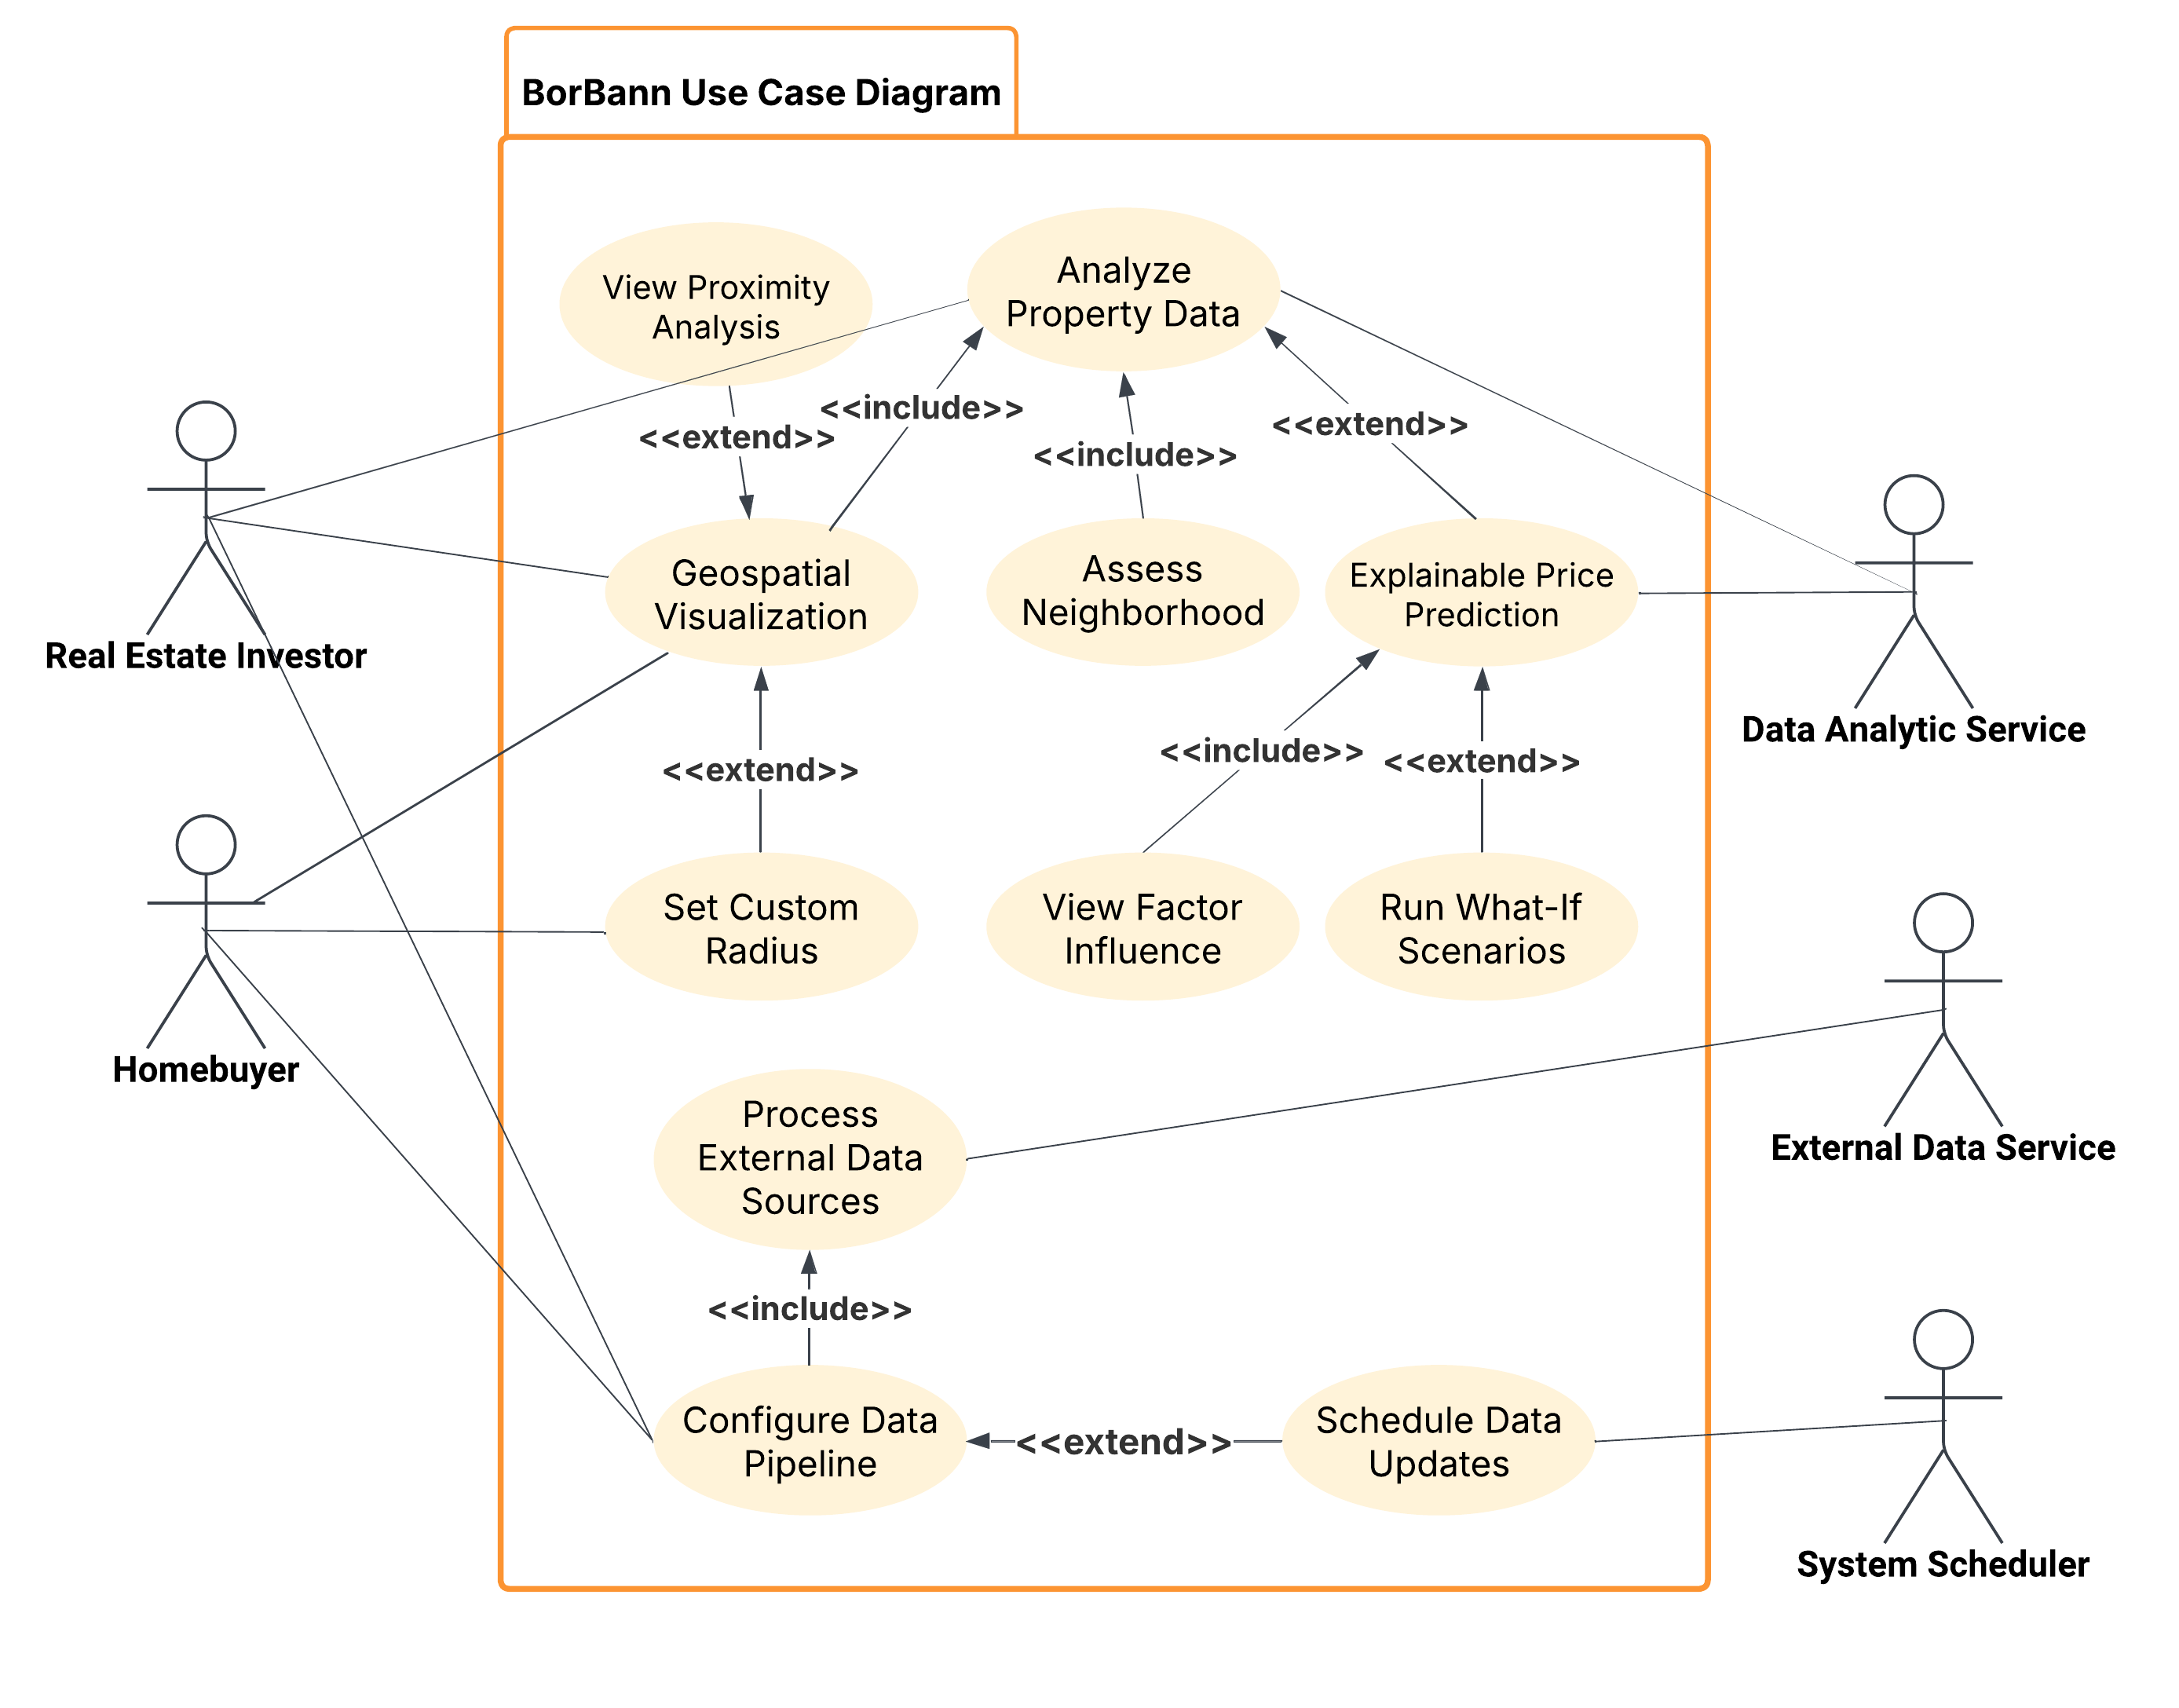
\includegraphics[width=0.8\textwidth]{assets/BorBann_Use_Case_Diagram.png}
	\caption{Use Case Diagram}
	\label{fig:use-case-diagram}
\end{figure}


\subsection{Primary Actors}

The use case diagram identifies five key actors interacting with the BorBann system:

\begin{itemize}
	\item \textbf{Real Estate Investor}  
	      Seeks in-depth property analytics, market trends, and investment decision support.
	      
	\item \textbf{Homebuyer}  
	      Interested in residential properties, lifestyle factors, and long-term value.
	      
	\item \textbf{Data Analytic Service}  
	      Provides analytic capabilities to support prediction and data analysis features.
	      
	\item \textbf{External Data Service}  
	      Supplies third-party data inputs via APIs and other integrations.
	      
	\item \textbf{System Scheduler}  
	      Automates routine system tasks such as scheduled data refresh operations.
\end{itemize}

\subsection{Core Use Cases}

The BorBann platform provides the following primary functionalities:

\begin{itemize}
	\item \textbf{Analyze Property Data}  
	      Allows users to examine detailed property information, metrics, and comparisons.  
	      \begin{itemize}
	      	\item \textit{Includes:} Assess Neighborhood
	      	\item \textit{Extended by:} Explainable Price Prediction
	      \end{itemize}
	      
	\item \textbf{Geospatial Visualization}  
	      Interactive map-based visualization of property and neighborhood data.  
	      \begin{itemize}
	      	\item \textit{Extended by:} Set Custom Radius, View Proximity Analysis
	      \end{itemize}
	      
	\item \textbf{Assess Neighborhood}  
	      Evaluates contextual factors around properties (e.g., schools, amenities).  
	      \begin{itemize}
	      	\item \textit{Includes:} View Factor Influence
	      	\item \textit{Extended by:} Check Environmental Risks
	      \end{itemize}
	      
	\item \textbf{Explainable Price Prediction}  
	      AI-generated pricing insights with interpretable influencing factors.  
	      \begin{itemize}
	      	\item \textit{Includes:} View Factor Influence
	      \end{itemize}
	      
	\item \textbf{Configure Data Pipeline}  
	      Enables setup of automated ingestion of external data from APIs and sources.  
	      \begin{itemize}
	      	\item \textit{Includes:} Process External Data Sources
	      	\item \textit{Extended by:} Schedule Data Updates
	      \end{itemize}
\end{itemize}

\subsection{Extended Functionality}

The following optional use cases extend the platform’s functionality:

\begin{itemize}
	\item \textbf{View Proximity Analysis}  
	      Triggered when users want detailed proximity-based data (e.g., nearby schools, transport).
	      
	\item \textbf{Set Custom Radius}  
	      Adds user-defined range settings for map-based filtering and analysis.
	      
	\item \textbf{Schedule Data Updates}  
	      Automates periodic refreshes of data pipelines using system scheduler logic.
	      
	\item \textbf{Check Environmental Risks}  
	      Enables users to access data on environmental threats (e.g., flood zones, pollution).
\end{itemize}

\subsection{Actor-System Interactions}

Each actor interacts with the system in distinct ways, as shown in the diagram:

\begin{itemize}
	\item \textbf{Real Estate Investor}
	      \begin{itemize}
	      	\item Initiates \textit{Analyze Property Data}, \textit{Geospatial Visualization}, and \textit{Configure Data Pipeline}
	      	\item Benefits from extended insights like \textit{Set Custom Radius}, \textit{View Proximity Analysis}, and \textit{Explainable Price Prediction}
	      \end{itemize}
	      
	\item \textbf{Homebuyer}
	      \begin{itemize}
	      	\item Accesses \textit{Analyze Property Data}, \textit{Geospatial Visualization}, \textit{Assess Neighborhood}, and \textit{Explainable Price Prediction}
	      	\item Makes use of neighborhood-specific features like \textit{View Factor Influence} and \textit{Check Environmental Risks}
	      \end{itemize}
	      
	\item \textbf{Data Analytic Service}
	      \begin{itemize}
	      	\item Collaborates with the system to enable \textit{Explainable Price Prediction}
	      \end{itemize}
	      
	\item \textbf{External Data Service}
	      \begin{itemize}
	      	\item Supports \textit{Process External Data Sources} as part of the data ingestion workflow
	      \end{itemize}
	      
	\item \textbf{System Scheduler}
	      \begin{itemize}
	      	\item Triggers \textit{Schedule Data Updates} as an automated background process
	      \end{itemize}
\end{itemize}

\subsection{Use Case Relationships}

\begin{itemize}
	\item \textbf{\textless{}\textless{}include\textgreater{}\textgreater{}}  
	      Represents mandatory sub-functions:
	      \begin{itemize}
	      	\item \textit{View Factor Influence} is included in both \textit{Assess Neighborhood} and \textit{Explainable Price Prediction}
	      	\item \textit{Process External Data Sources} is included in \textit{Configure Data Pipeline}
	      \end{itemize}
	      
	\item \textbf{\textless{}\textless{}extend\textgreater{}\textgreater{}}  
	      Represents optional or conditional behavior:
	      \begin{itemize}
	      	\item \textit{Set Custom Radius} and \textit{View Proximity Analysis} extend \textit{Geospatial Visualization}
	      	\item \textit{Check Environmental Risks} extends \textit{Assess Neighborhood}
	      	\item \textit{Schedule Data Updates} extends \textit{Configure Data Pipeline}
	      \end{itemize}
\end{itemize}

%----------------------------------------------------------------------
\section{Use Case Model}
%----------------------------------------------------------------------

The Use Case Model details the interactions depicted in the Use Case Diagram, describing each use case within BorBann's core features.

% \begin{table}[htbp]
%   \centering
%   \renewcommand{\arraystretch}{1.3}
%   \begin{tabular}{|>{\columncolor[gray]{0.95}}p{0.25\textwidth}|p{0.65\textwidth}|}
%     \hline
%     \rowcolor[gray]{0.9} \textbf{Use Case Name} & \textbf{Search Properties \& Listings}                                                                  \\
%     \hline
%     \textbf{Actors}                             & Real Estate Investor, Homebuyer, Property Developer                                                     \\
%     \hline
%     \textbf{Description}                        & Allows users to search for properties based on various criteria and view results in a structured format \\
%     \hline
%     \textbf{Preconditions}                      & User is logged into the system                                                                          \\
%     \hline
%     \textbf{Basic Flow}                         &
%     \begin{enumerate}
%       \item User accesses the search interface
%       \item System presents search filters (included use case)
%       \item User enters search criteria
%       \item System processes the search query
%       \item System displays matching properties
%       \item User browses through results
%     \end{enumerate} \\
%     \hline
%     \textbf{Alternative Flows}                  &
%     \begin{itemize}
%       \item User can refine search criteria if results are unsatisfactory
%       \item User can extend to compare properties
%       \item User can save search criteria for future use
%     \end{itemize} \\
%     \hline
%     \textbf{Postconditions}                     & User views a list of properties matching their criteria                                                 \\
%     \hline
%     \textbf{Associated Feature}                 & Automated Data Integration Pipeline - providing deduplicated listings from multiple sources             \\
%     \hline
%   \end{tabular}
%   \caption{Search Properties \& Listings Use Case}
%   \label{tab:search-use-case}
% \end{table}

\begin{table}[h]
	\centering
	\renewcommand{\arraystretch}{1.3}
	\begin{tabular}{|>{\columncolor[gray]{0.95}}p{0.25\textwidth}|p{0.65\textwidth}|}
		\hline
		\rowcolor[gray]{0.9} \textbf{Use Case Name} & \textbf{View Property Insights}                                                                  \\
		\hline
		\textbf{Actors}                             & Real Estate Investor, Homebuyer, Property Developer                                              \\
		\hline
		\textbf{Description}                        & Provides users with comprehensive analytics and contextual information about specific properties \\
		\hline
		\textbf{Preconditions}                      & User has selected a property from search results                                                 \\
		\hline
		\textbf{Basic Flow}                         &                                                                                                  
		\begin{enumerate}
		\item User selects a property for detailed viewing
		\item System retrieves comprehensive property data
		\item System presents property details with analytics
		\item System displays neighborhood characteristics
		\item System shows historical performance metrics
		\item User reviews information
		\end{enumerate} \\
		\hline
		\textbf{Alternative Flows}                  &                                                                                                  
		\begin{itemize}
		\item User can extend to save the property as a favorite
		\item User can extend to view explainable price predictions
		\item User can request additional specific analytics
		\end{itemize} \\
		\hline
		\textbf{Postconditions}                     & User gains comprehensive insights about the property                                             \\
		\hline
		\textbf{Associated Feature}                 & Local Contextual Analytics - providing trend analysis and neighborhood-specific insights         \\
		\hline
	\end{tabular}
	\caption{View Property Insights Use Case}
	\label{tab:insights-use-case}
\end{table}

\begin{table}[h]
	\centering
	\renewcommand{\arraystretch}{1.3}
	\begin{tabular}{|>{\columncolor[gray]{0.95}}p{0.25\textwidth}|p{0.65\textwidth}|}
		\hline
		\rowcolor[gray]{0.9} \textbf{Use Case Name} & \textbf{Explainable Price Prediction}                                                                    \\
		\hline
		\textbf{Actors}                             & Real Estate Investor, Homebuyer                                                                          \\
		\hline
		\textbf{Description}                        & Provides transparent, interpretable price predictions with detailed explanations of contributing factors \\
		\hline
		\textbf{Preconditions}                      & User is viewing property insights                                                                        \\
		\hline
		\textbf{Basic Flow}                         &                                                                                                          
		\begin{enumerate}
		\item User requests price prediction for a property
		\item System calculates predicted price using its models
		\item System generates explanation of factors influencing the prediction
		\item System presents prediction with confidence interval
		\item System displays factor weights and their impact
		\item User reviews prediction and explanation
		\end{enumerate} \\
		\hline
		\textbf{Alternative Flows}                  &                                                                                                          
		\begin{itemize}
		\item User can adjust factors to see impact on prediction
		\item User can compare prediction with market averages
		\item User can save prediction for future reference
		\end{itemize} \\
		\hline
		\textbf{Postconditions}                     & User understands the predicted price and the reasoning behind it                                         \\
		\hline
		\textbf{Associated Feature}                 & Explainable Price Prediction Model - providing transparent explanations for price predictions            \\
		\hline
	\end{tabular}
	\caption{Explainable Price Prediction Use Case}
	\label{tab:prediction-use-case}
\end{table}

% \begin{table}[htbp]
%   \centering
%   \renewcommand{\arraystretch}{1.3}
%   \begin{tabular}{|>{\columncolor[gray]{0.95}}p{0.25\textwidth}|p{0.65\textwidth}|}
%     \hline
%     \rowcolor[gray]{0.9} \textbf{Use Case Name} & \textbf{Geospatial Visualization}                                                                  \\
%     \hline
%     \textbf{Actors}                             & Real Estate Investor, Homebuyer                                                                    \\
%     \hline
%     \textbf{Description}                        & Enables users to visualize property and market data on interactive maps with various data overlays \\
%     \hline
%     \textbf{Preconditions}                      & User has access to the platform                                                                    \\
%     \hline
%     \textbf{Basic Flow}                         &
%     \begin{enumerate}
%       \item User accesses the map interface
%       \item System loads the base map with property markers
%       \item User selects desired data overlays (e.g., price heatmaps, transit lines)
%       \item System renders the selected overlays
%       \item User interacts with the map (zoom, pan, click)
%       \item System provides context-sensitive information based on interaction
%     \end{enumerate} \\
%     \hline
%     \textbf{Alternative Flows}                  &
%     \begin{itemize}
%       \item User can filter properties shown on the map
%       \item User can measure distances between points
%       \item User can switch between different base maps
%     \end{itemize} \\
%     \hline
%     \textbf{Postconditions}                     & User visualizes spatial relationships and patterns relevant to their needs                         \\
%     \hline
%     \textbf{Associated Feature}                 & Geospatial Visualization - providing interactive maps with data overlays and proximity analysis    \\
%     \hline
%   \end{tabular}
%   \caption{Geospatial Visualization Use Case}
%   \label{tab:geospatial-use-case}
% \end{table}

\clearpage
%======================================================================
\section{User Interface Design}
%======================================================================

\begin{figure}[htbp]
	\centering
	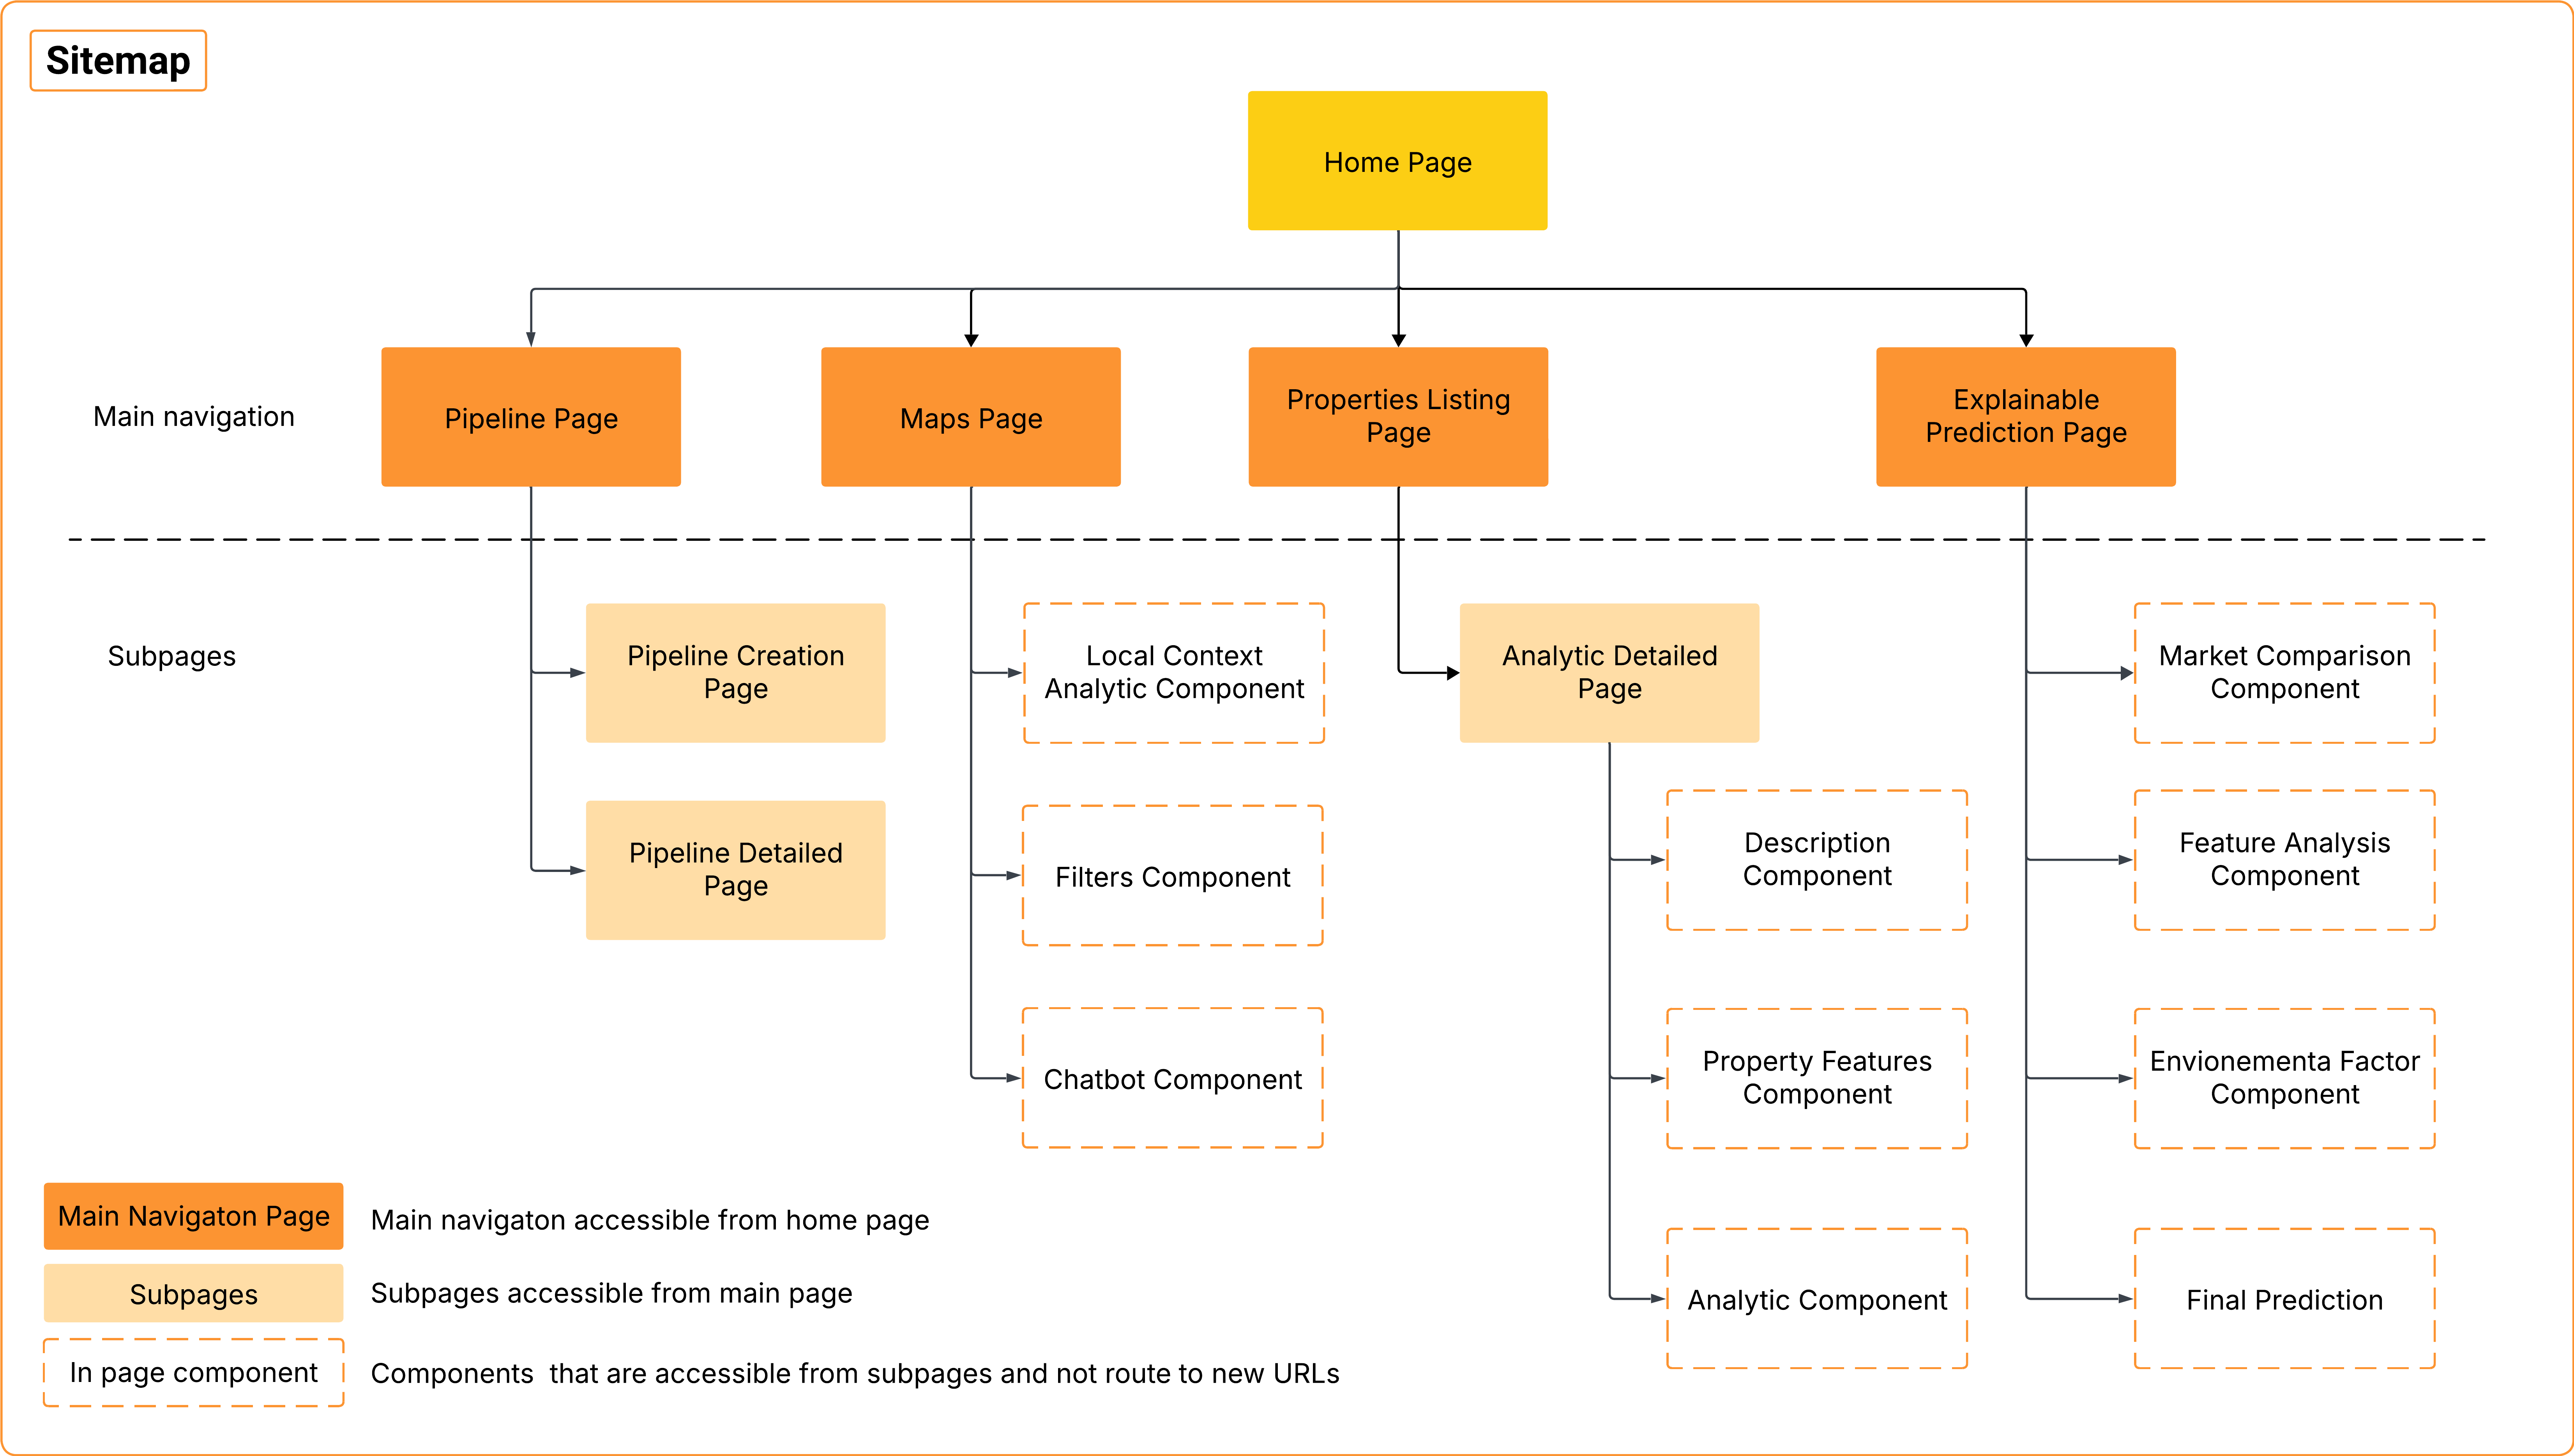
\includegraphics[width=1\textwidth]{assets/sitemap.png}
	\caption{Sitemap - Platform Structure Overview}
	\label{fig:sitemap}
\end{figure}

\noindent Figure \ref{fig:sitemap} shows the structure of the BorBann platform. The Home Page acts as the central access point leading to four main sections: Pipeline, Maps, Properties Listing, and Explainable Prediction pages. 

Each main section connects to specific subpages. The Pipeline section includes Creation and Detailed pages. The Maps section features Local Context Analytics, Filters, and Chatbot components. The Properties section provides Analytic Detailed pages with Description, Property Features, and Analytics components. The Explainable Prediction section offers Market Comparison, Feature Analysis, Environmental Factor analysis, and Final Prediction components.

This structure organizes the platform's key functions in a logical flow, making it easy for users to navigate between data management, visualization, and prediction features.

\pagebreak
%======================================================================

\begin{figure}[htbp]
  \centering
  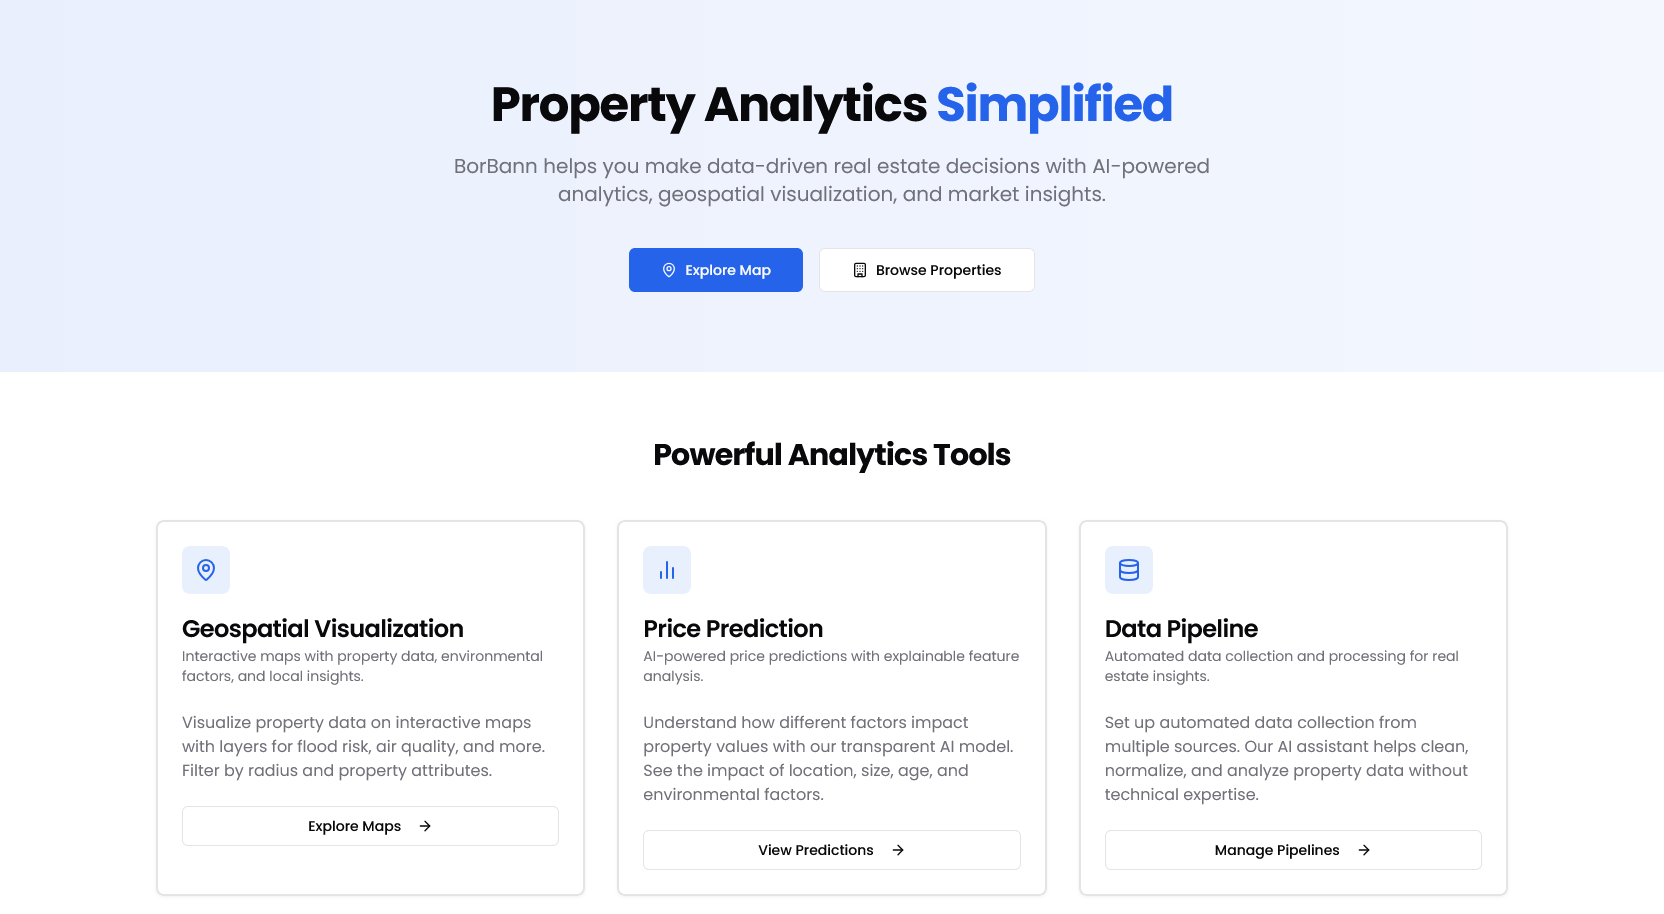
\includegraphics[width=1\textwidth]{assets/ui/homepage.png}
  \caption{BorBann Platform Homepage}
  \label{fig:homepage}
\end{figure}

Figure \ref{fig:homepage} shows the BorBann platform homepage, which provides an intuitive entry point to the system. The page presents the core value proposition with "Property Analytics Simplified" and briefly explains how BorBann helps users make data-driven real estate decisions through analytics, geospatial visualization, and market insights. Two primary action buttons - "Explore Map" and "Browse Properties" - enable quick access to key functionality. The lower section showcases three main analytics tools: Geospatial Visualization for interactive property mapping, Price Prediction with explainable AI features, and Data Pipeline for automated data collection and processing.

%======================================================================
\pagebreak
\begin{figure}[h]
\centering
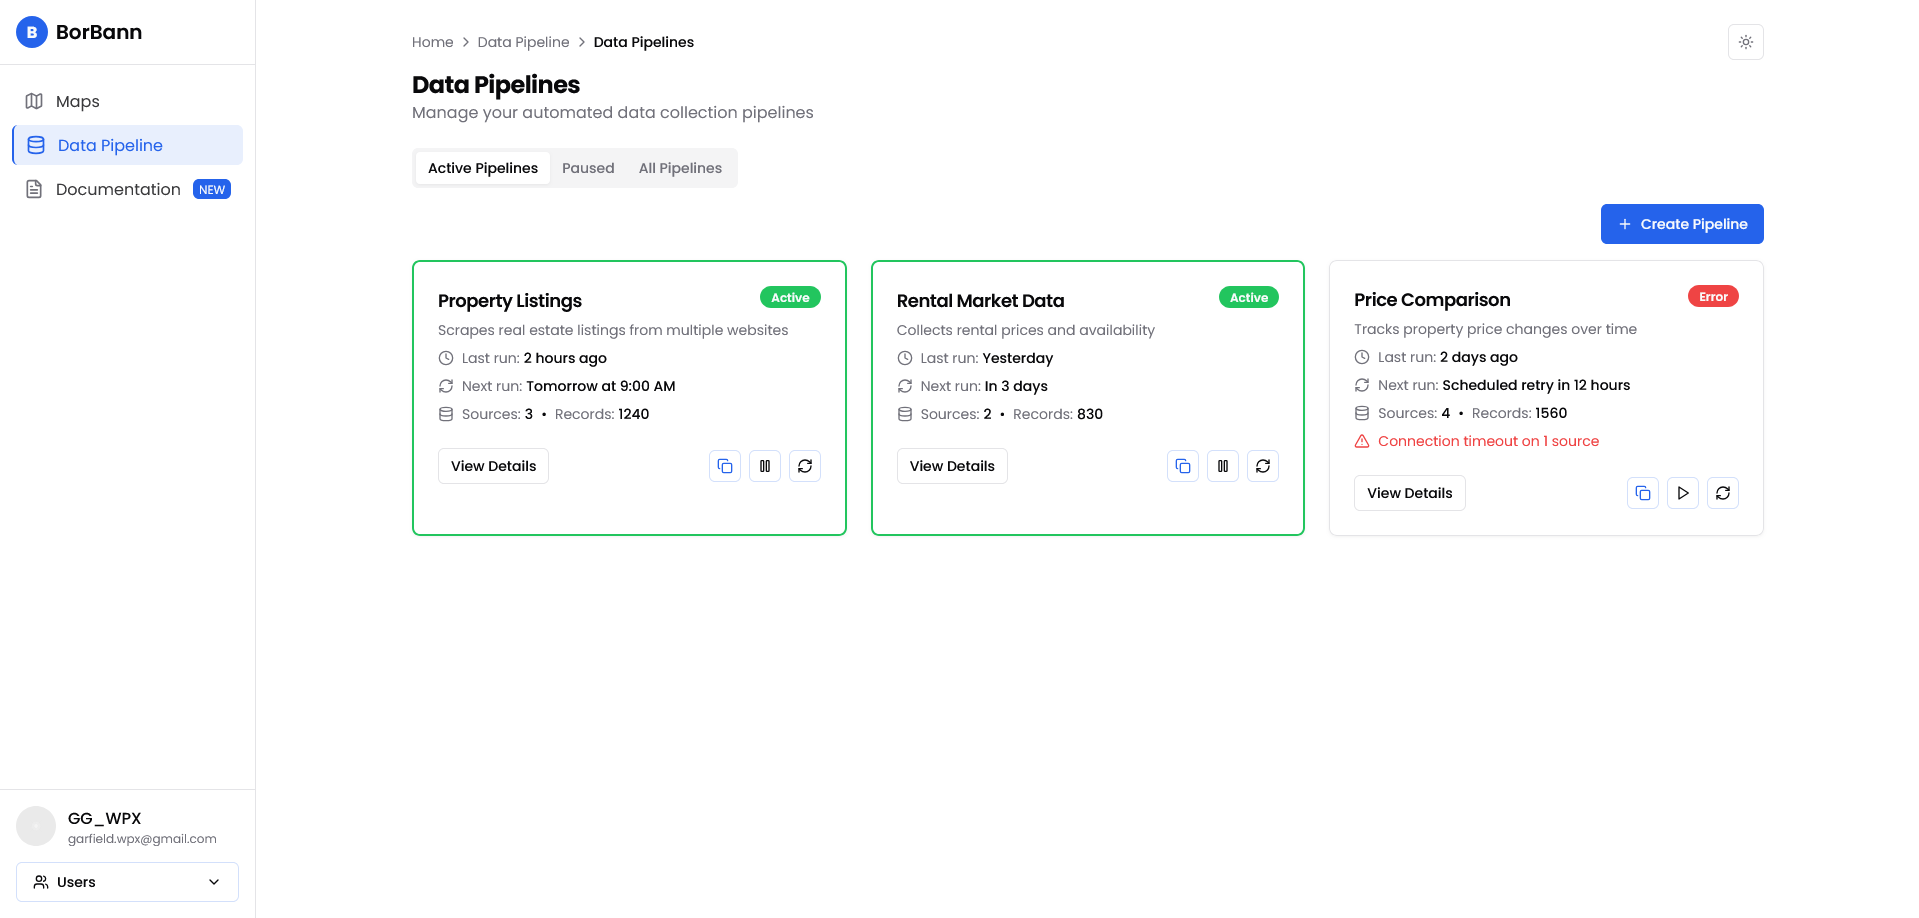
\includegraphics[width=1\textwidth]{assets/ui/data-pipelines-main.png}
\caption{Data Pipeline Management Interface}
\label{fig:data-pipelines}
\end{figure}

Figure \ref{fig:data-pipelines} showcases the Data Pipeline management dashboard, providing users with comprehensive control over their automated data collection processes. The interface features intuitive navigation with filtering options for Active, Paused, and All Pipelines, enabling efficient workflow management.

Each pipeline card presents essential operational metrics including last run timestamp, next scheduled execution, number of data sources, and total records processed. This at-a-glance view allows users to quickly assess data freshness and monitor collection performance across multiple pipelines.

\begin{figure}[h]
\centering
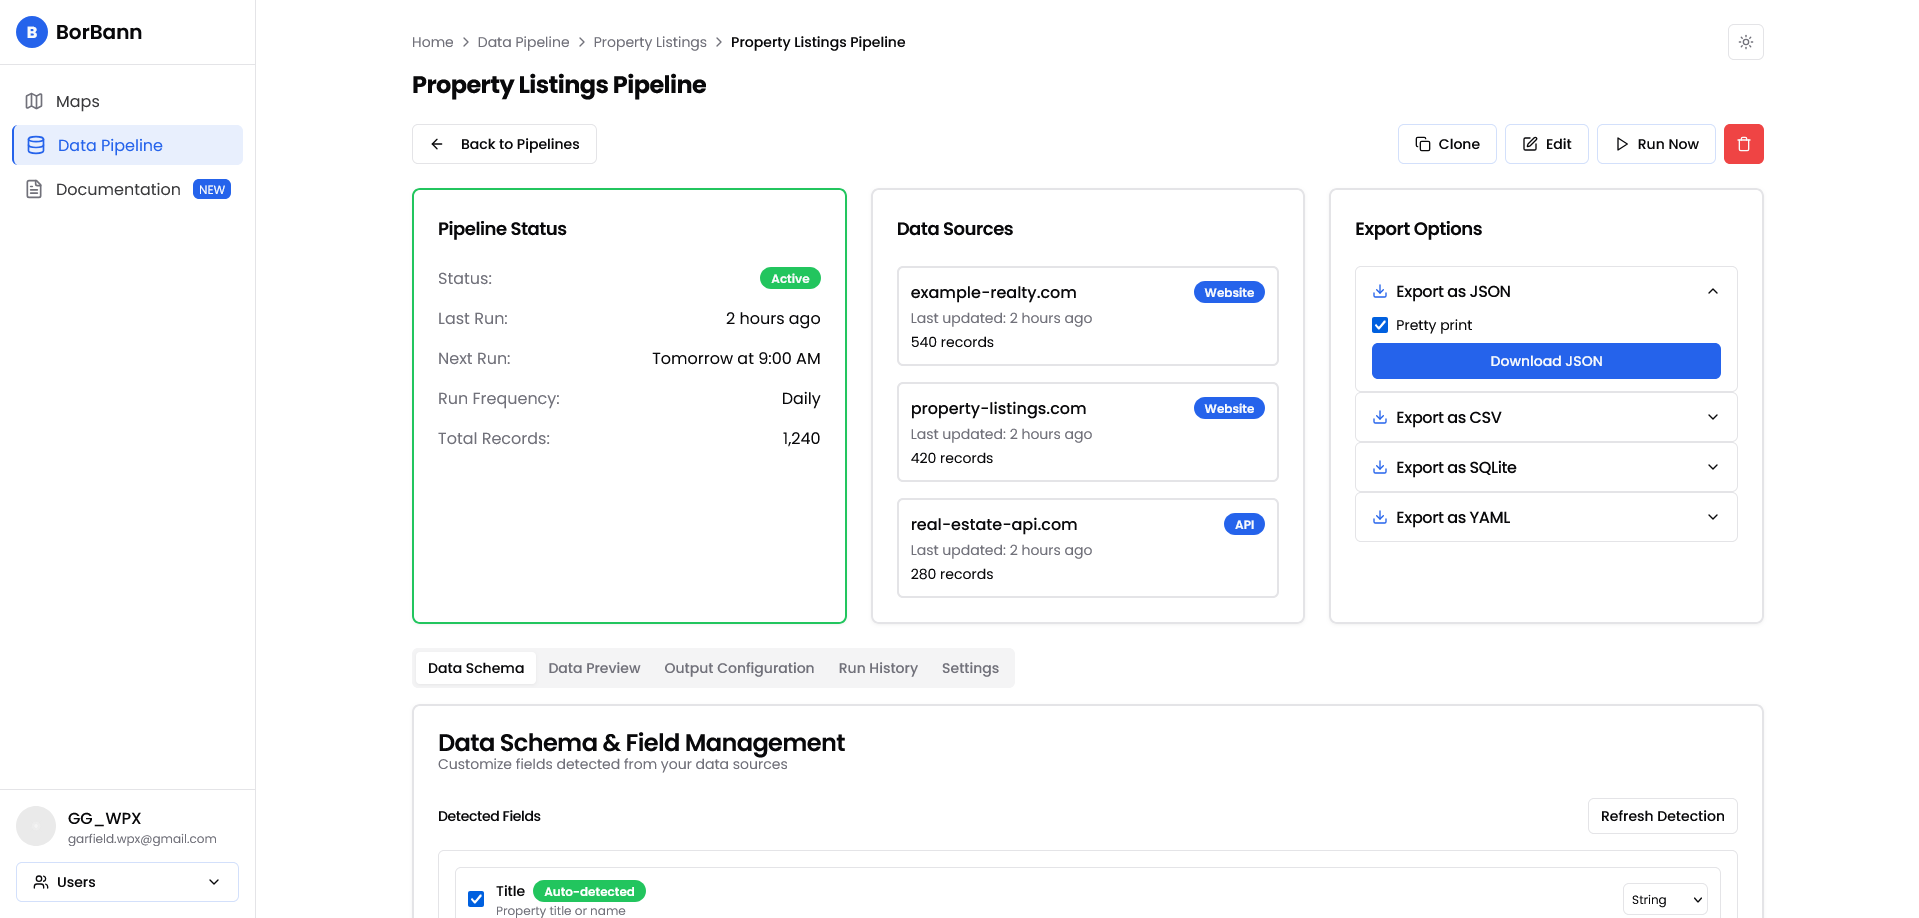
\includegraphics[width=1\textwidth]{assets/ui/data-pipelines-detailed-1.png}
\caption{Data Integration Pipeline Detail - Overview}
\label{fig:data-pipelines-detailed-1}
\end{figure}

Figure \ref{fig:data-pipelines-detailed-1} illustrates the pipeline detail view, highlighting key operational components including current status indicators, connected data sources, and available export formats. This overview provides users with immediate visibility into pipeline configuration and functionality.

\begin{figure}[h]
\centering
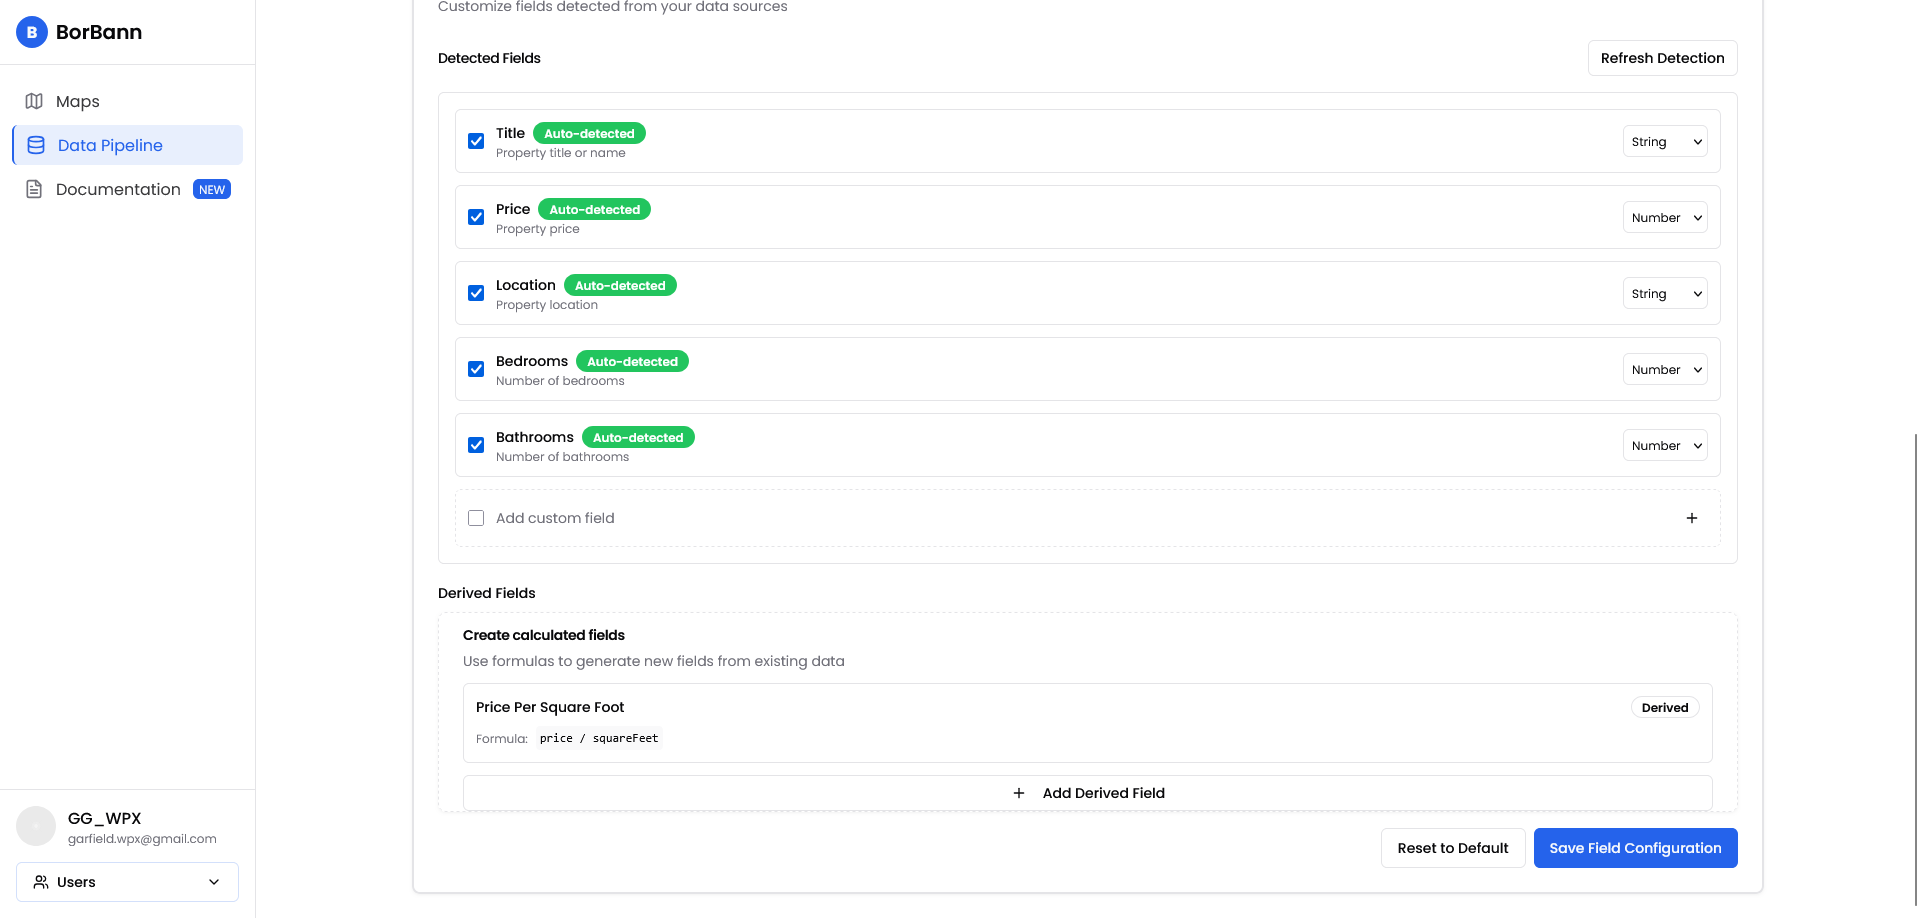
\includegraphics[width=1\textwidth]{assets/ui/data-pipelines-detailed-2.png}
\caption{Data Integration Pipeline Detail - Field Management}
\label{fig:data-pipelines-detailed-2}
\end{figure}

Figure \ref{fig:data-pipelines-detailed-2} displays the field management section of the pipeline detail page. This interface empowers users to customize their data structure by managing output fields and creating derived fields through a visual formula builder. Users can transform raw data into meaningful metrics without writing code.

\begin{figure}[h]
\centering
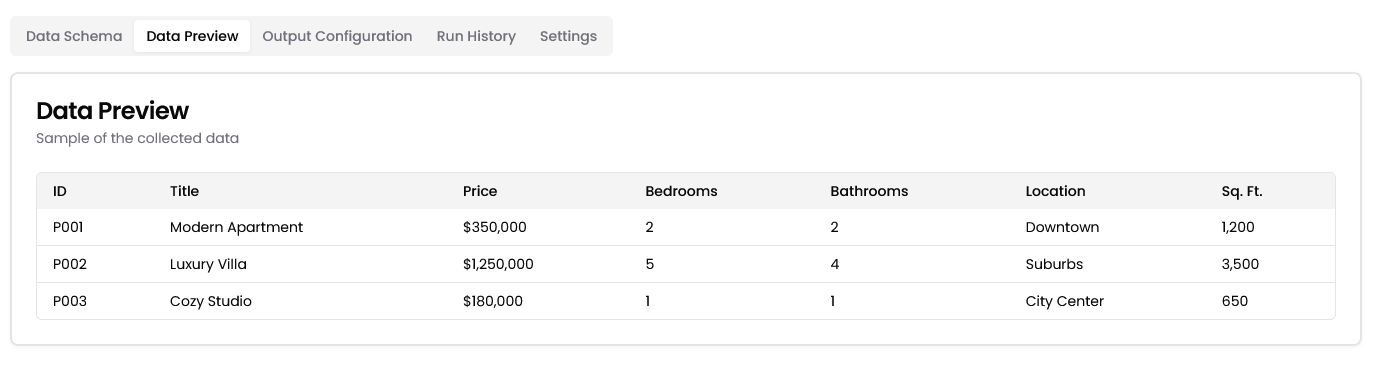
\includegraphics[width=1\textwidth]{assets/ui/data-pipelines-detailed-data-preview.png}
\caption{Data Integration Pipeline Detail - Output Data Preview}
\label{fig:data-pipelines-detailed-data-preview}
\end{figure}

Figure \ref{fig:data-pipelines-detailed-data-preview} presents the data preview tab, where users can examine sample records generated by their pipeline. This real-time preview functionality allows users to validate data quality and structure before export or analysis.

\pagebreak
\begin{figure}[h]
\centering
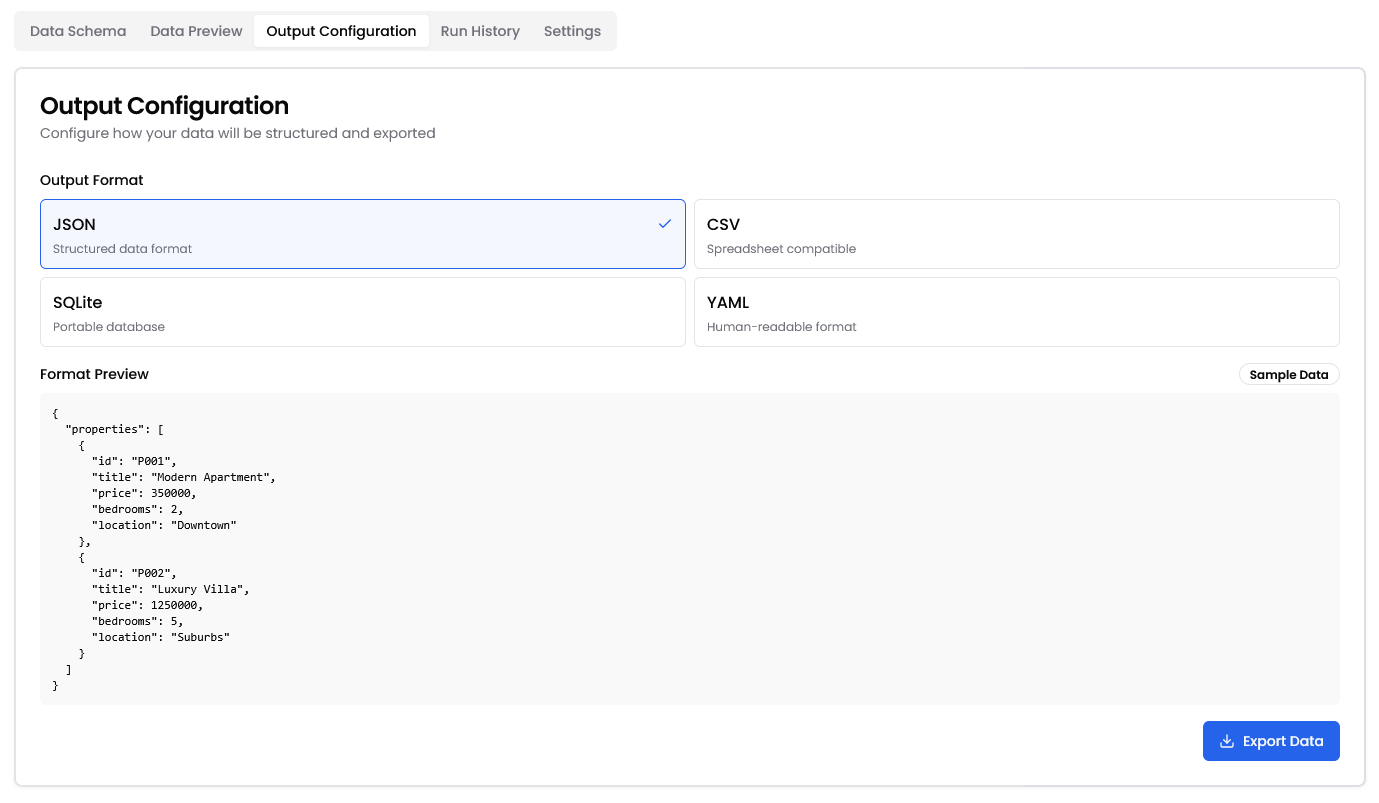
\includegraphics[width=1\textwidth]{assets/ui/data-pipelines-detailed-export-data.png}
\caption{Data Integration Pipeline Detail - Export Configuration}
\label{fig:data-pipelines-detailed-export-data}
\end{figure}

Figure \ref{fig:data-pipelines-detailed-export-data} shows the export configuration interface, where users can precisely define output schemas for their data exports. This tab enables users to select specific fields, customize formatting, and choose from multiple export formats to meet their downstream requirements.

\begin{figure}[h]
\centering
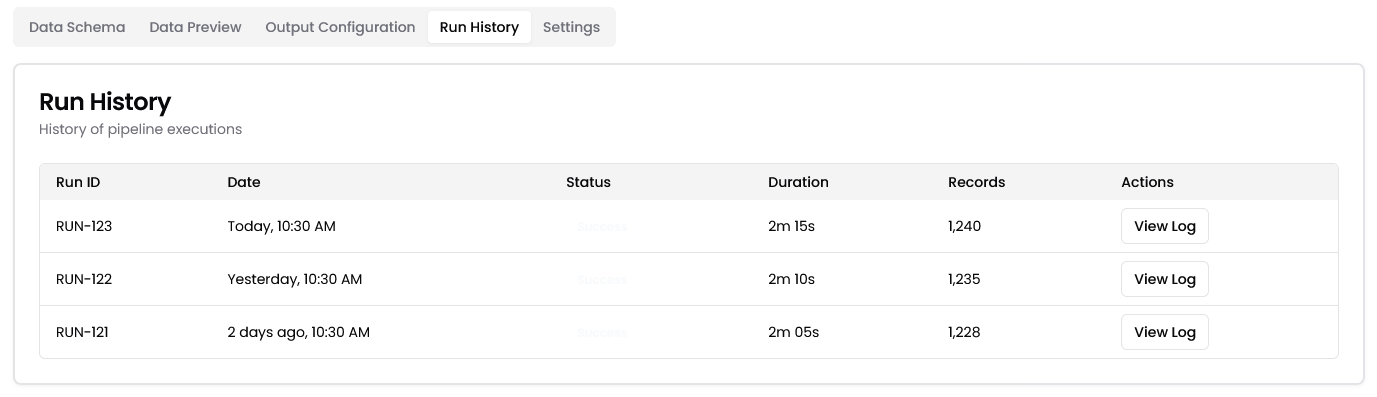
\includegraphics[width=1\textwidth]{assets/ui/data-pipelines-detailed-run-history.png}
\caption{Data Integration Pipeline Detail - Run History}
\label{fig:data-pipelines-detailed-run-history}
\end{figure}

Figure \ref{fig:data-pipelines-detailed-run-history} displays the run history tab, providing a chronological log of pipeline executions. This audit trail includes execution timestamps, duration metrics, and status indicators, enabling users to monitor performance trends and troubleshoot any execution issues.

\begin{figure}[h]
\centering
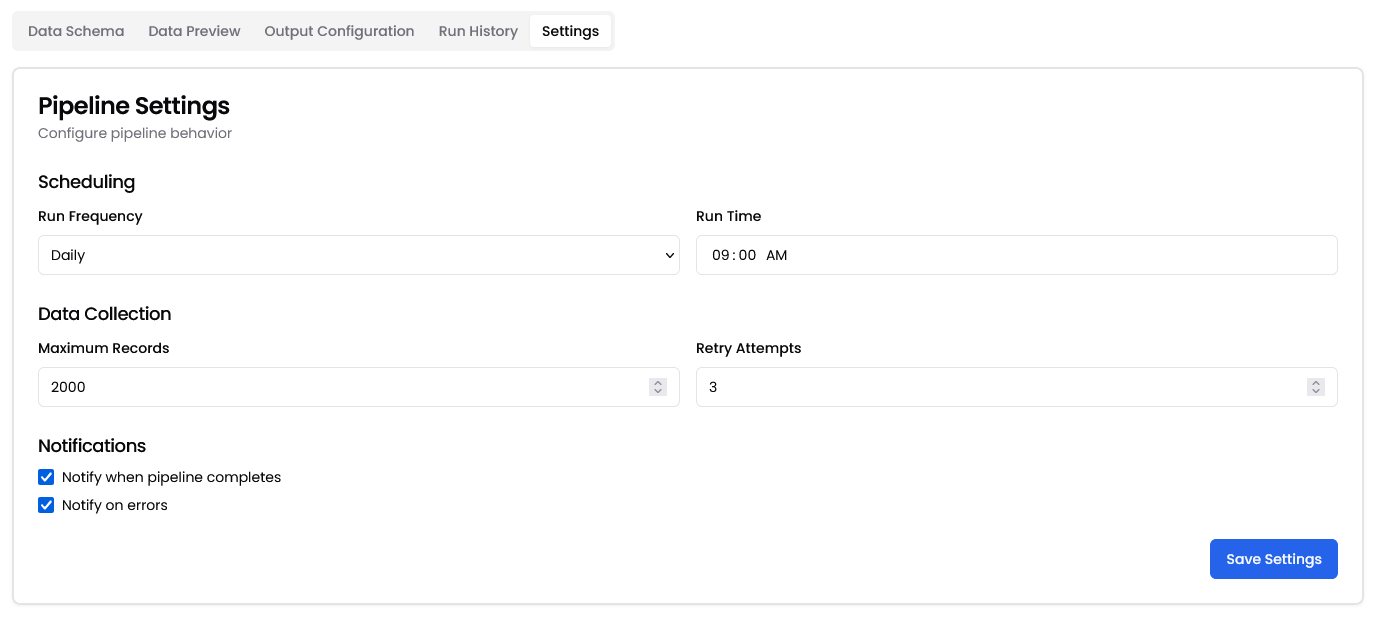
\includegraphics[width=1\textwidth]{assets/ui/data-pipelines-detailed-pipeline-setting.png}
\caption{Data Integration Pipeline Detail - Pipeline Settings}
\label{fig:data-pipelines-detailed-pipeline-setting}
\end{figure}

\pagebreak
Figure \ref{fig:data-pipelines-detailed-pipeline-setting} illustrates the pipeline settings tab, where users can configure automation parameters including execution schedules, notification preferences, and retry policies. These controls allow users to establish reliable data collection routines that align with their operational requirements.

\begin{figure}[h]
\centering
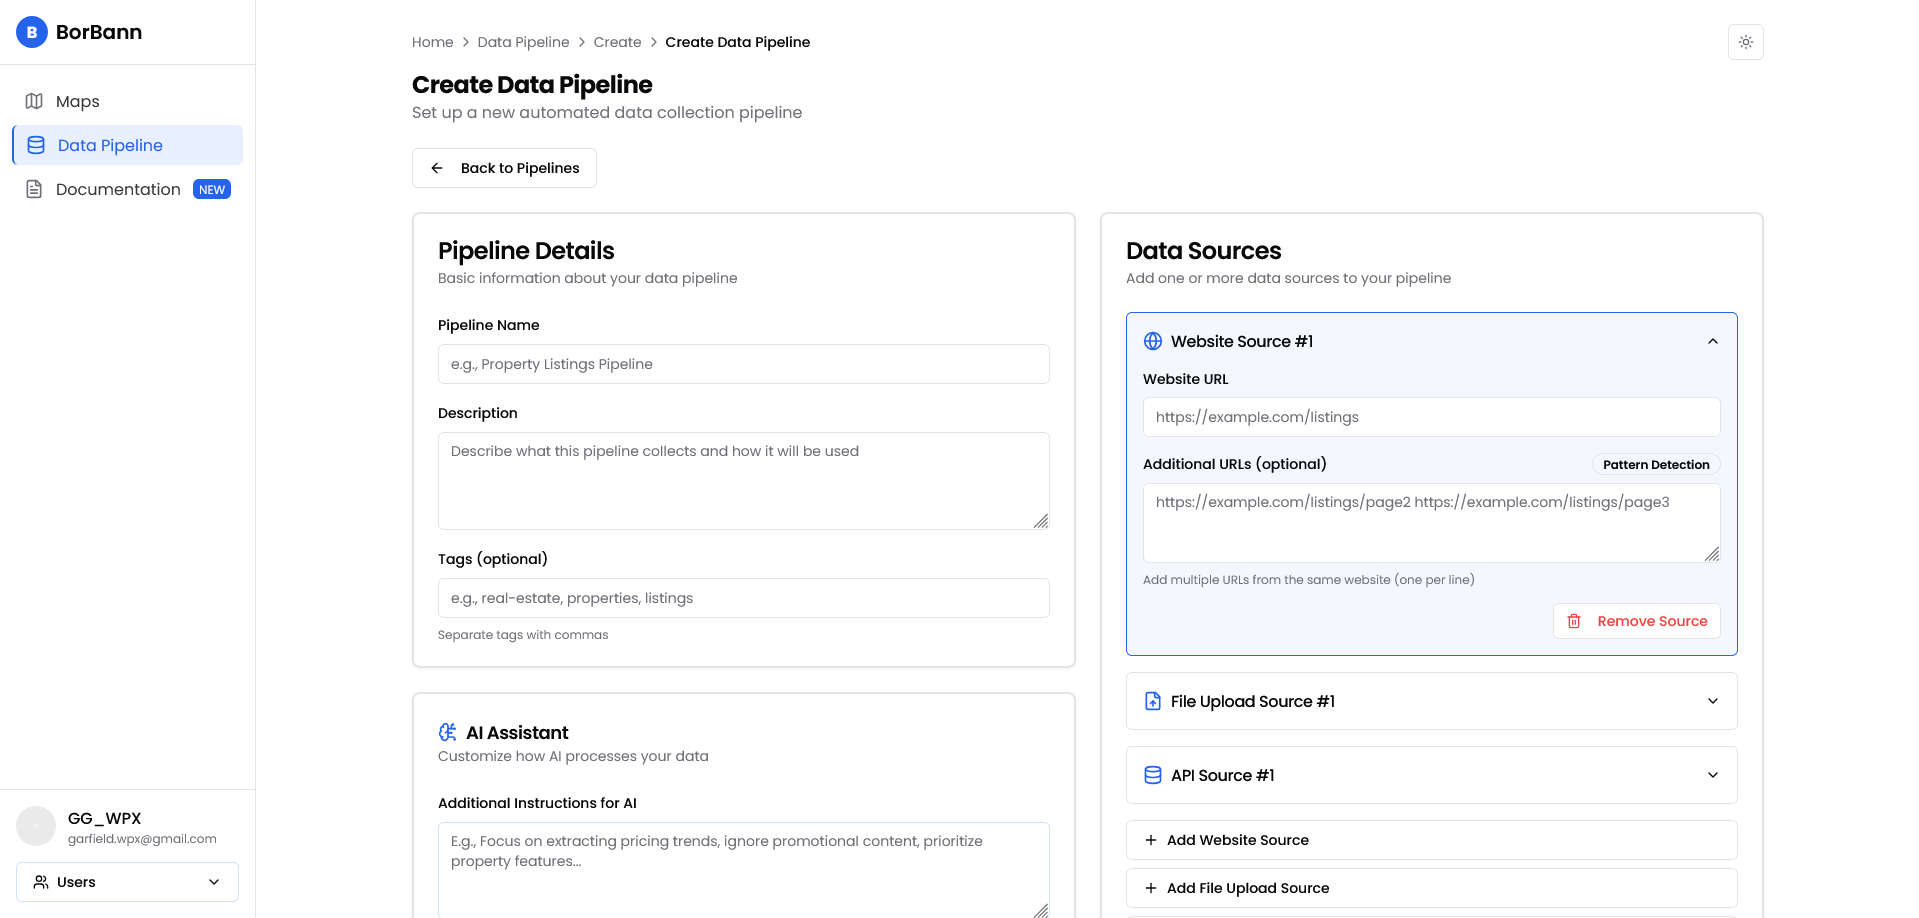
\includegraphics[width=1\textwidth]{assets/ui/data-pipelines-create.png}
\caption{Data Integration Pipeline - Creation Interface}
\label{fig:data-pipelines-create-1}
\end{figure}

Figure \ref{fig:data-pipelines-create-1} shows the pipeline creation interface where users input website URLs for automated data extraction. The form enables non-technical users to configure scraping operations without coding knowledge.

\begin{figure}[h]
\centering
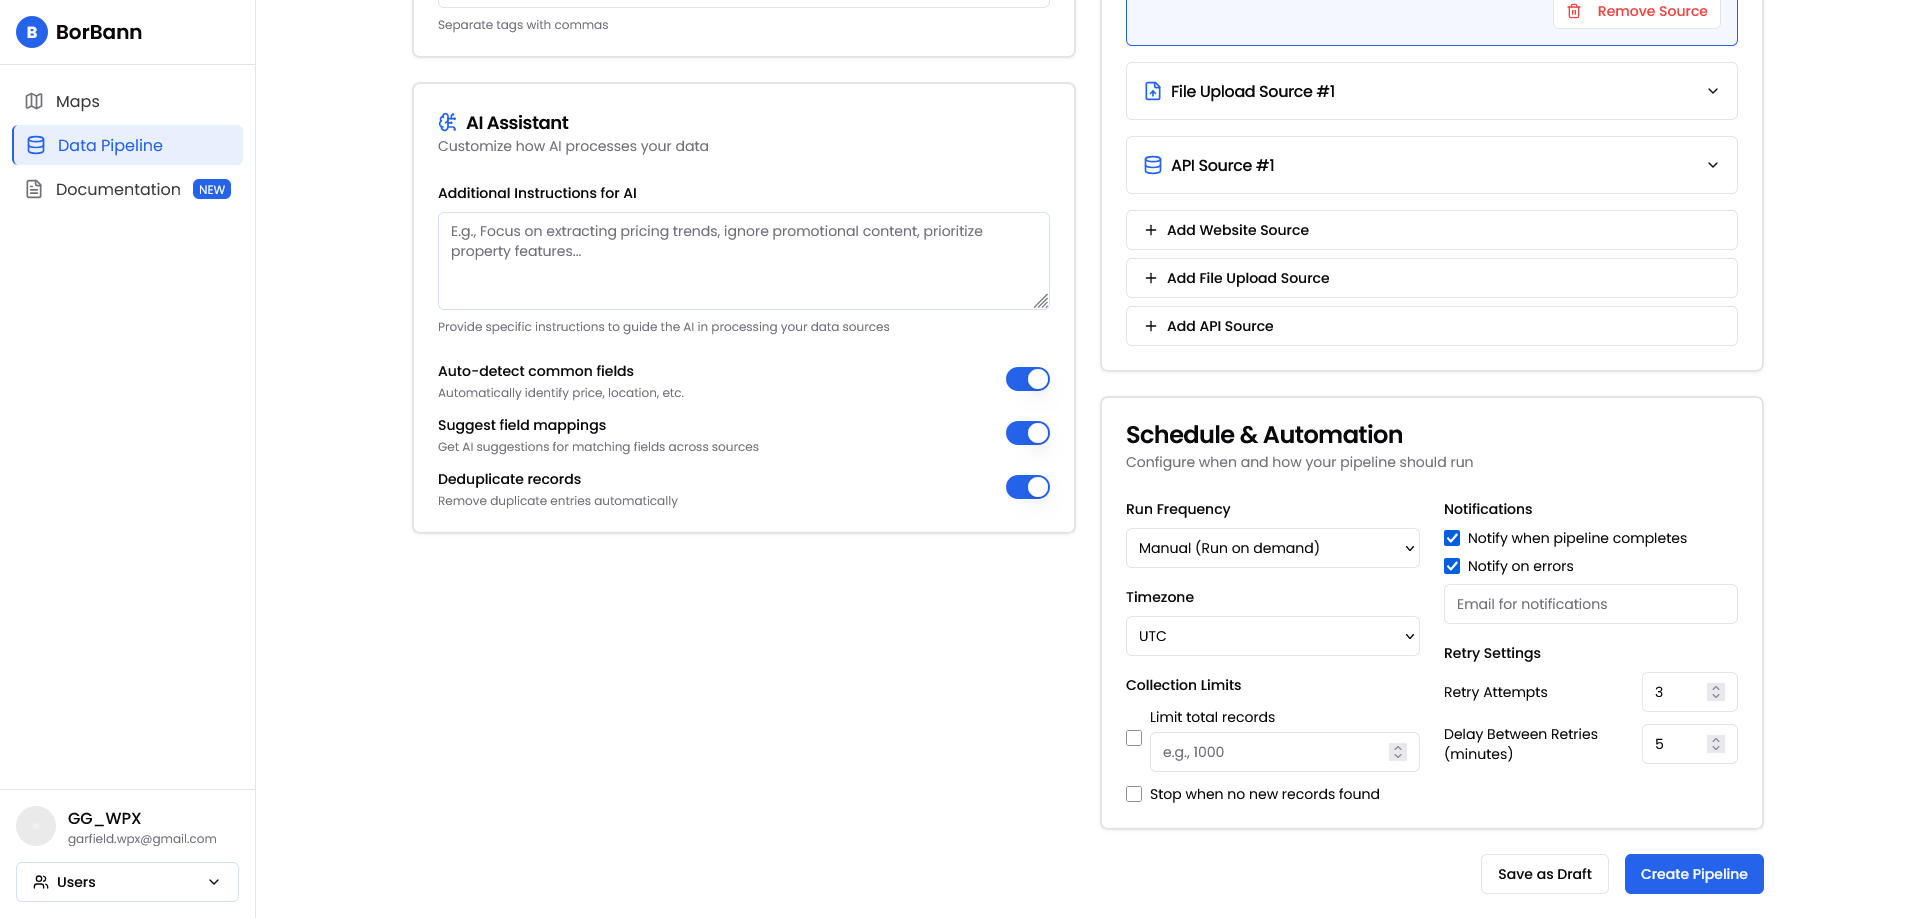
\includegraphics[width=1\textwidth]{assets/ui/data-pipelines-create-2.png}
\caption{Data Integration Pipeline - Advanced Configuration and Scheduling}
\label{fig:data-pipelines-create-2}
\end{figure}

Figure \ref{fig:data-pipelines-create-2} displays automation settings for pipeline execution with scheduling options and AI-assisted extraction configuration. Users can set run frequency and notification preferences to maintain automated data collection.

\begin{figure}[h]
\centering
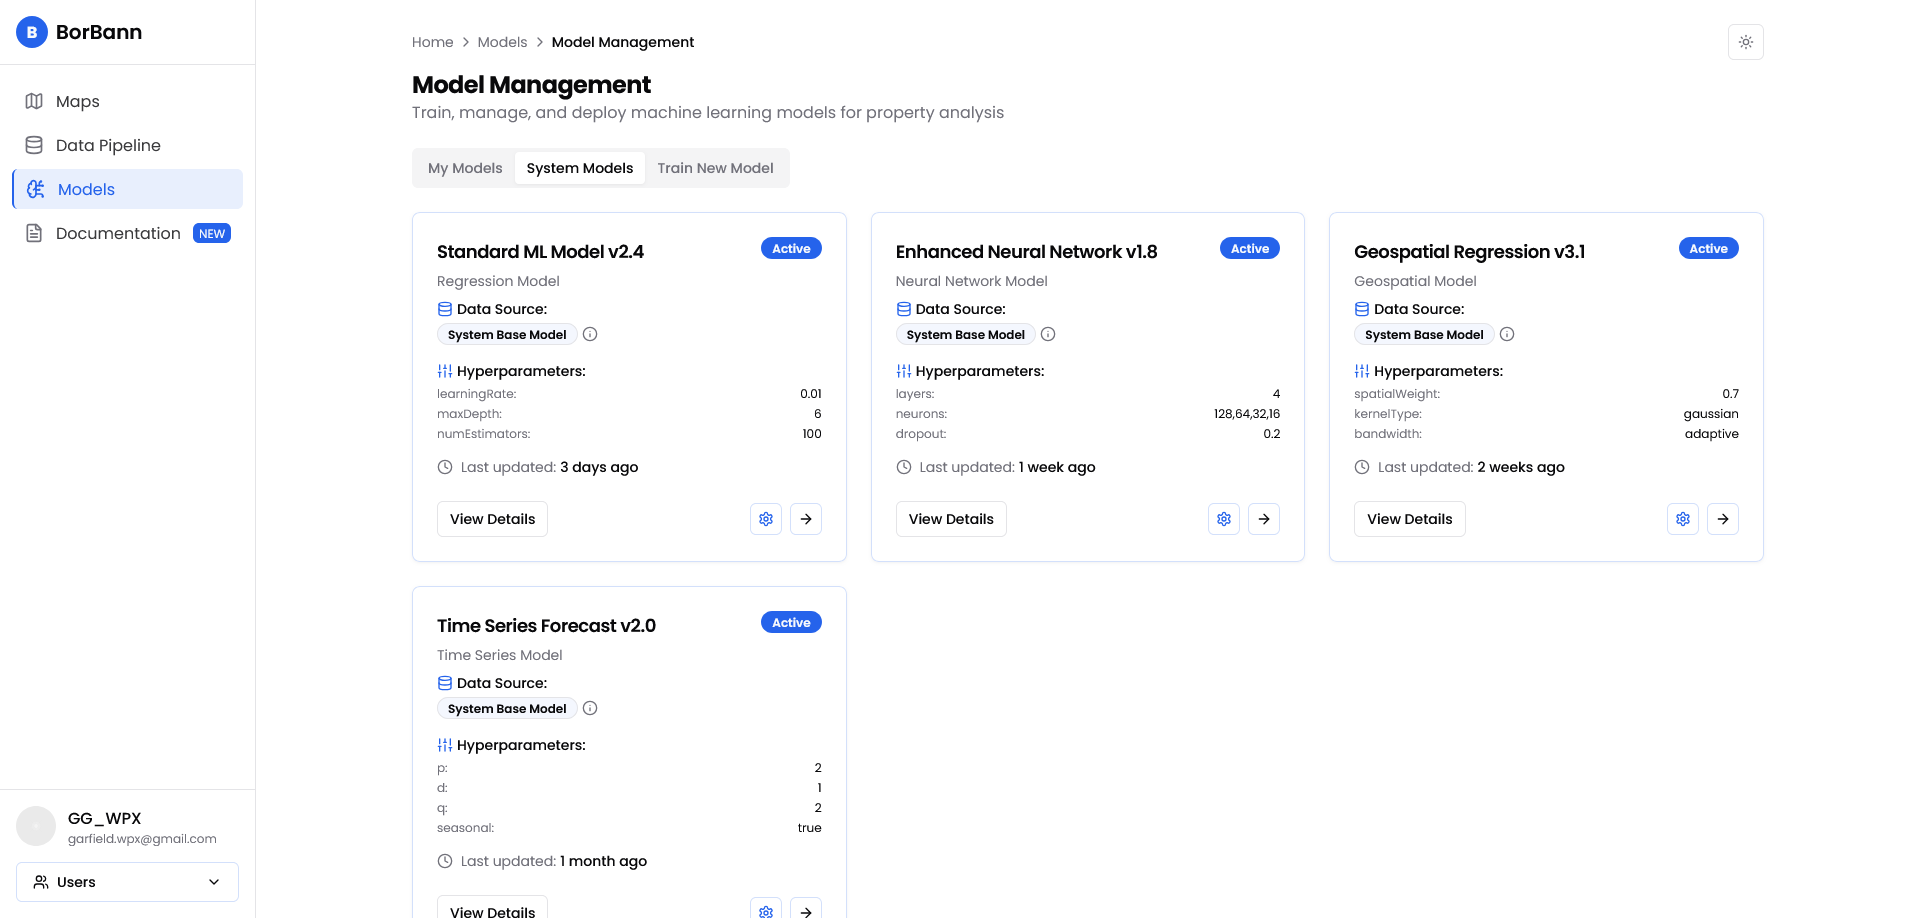
\includegraphics[width=1\textwidth]{assets/ui/models-models-list.png}
\caption{Model Management Dashboard}
\label{fig:models-models-list}
\end{figure}

Figure \ref{fig:models-models-list} presents the model management dashboard where users can view and control prediction models. The interface displays performance metrics and allows single-click model activation.

\begin{figure}[h]
\centering
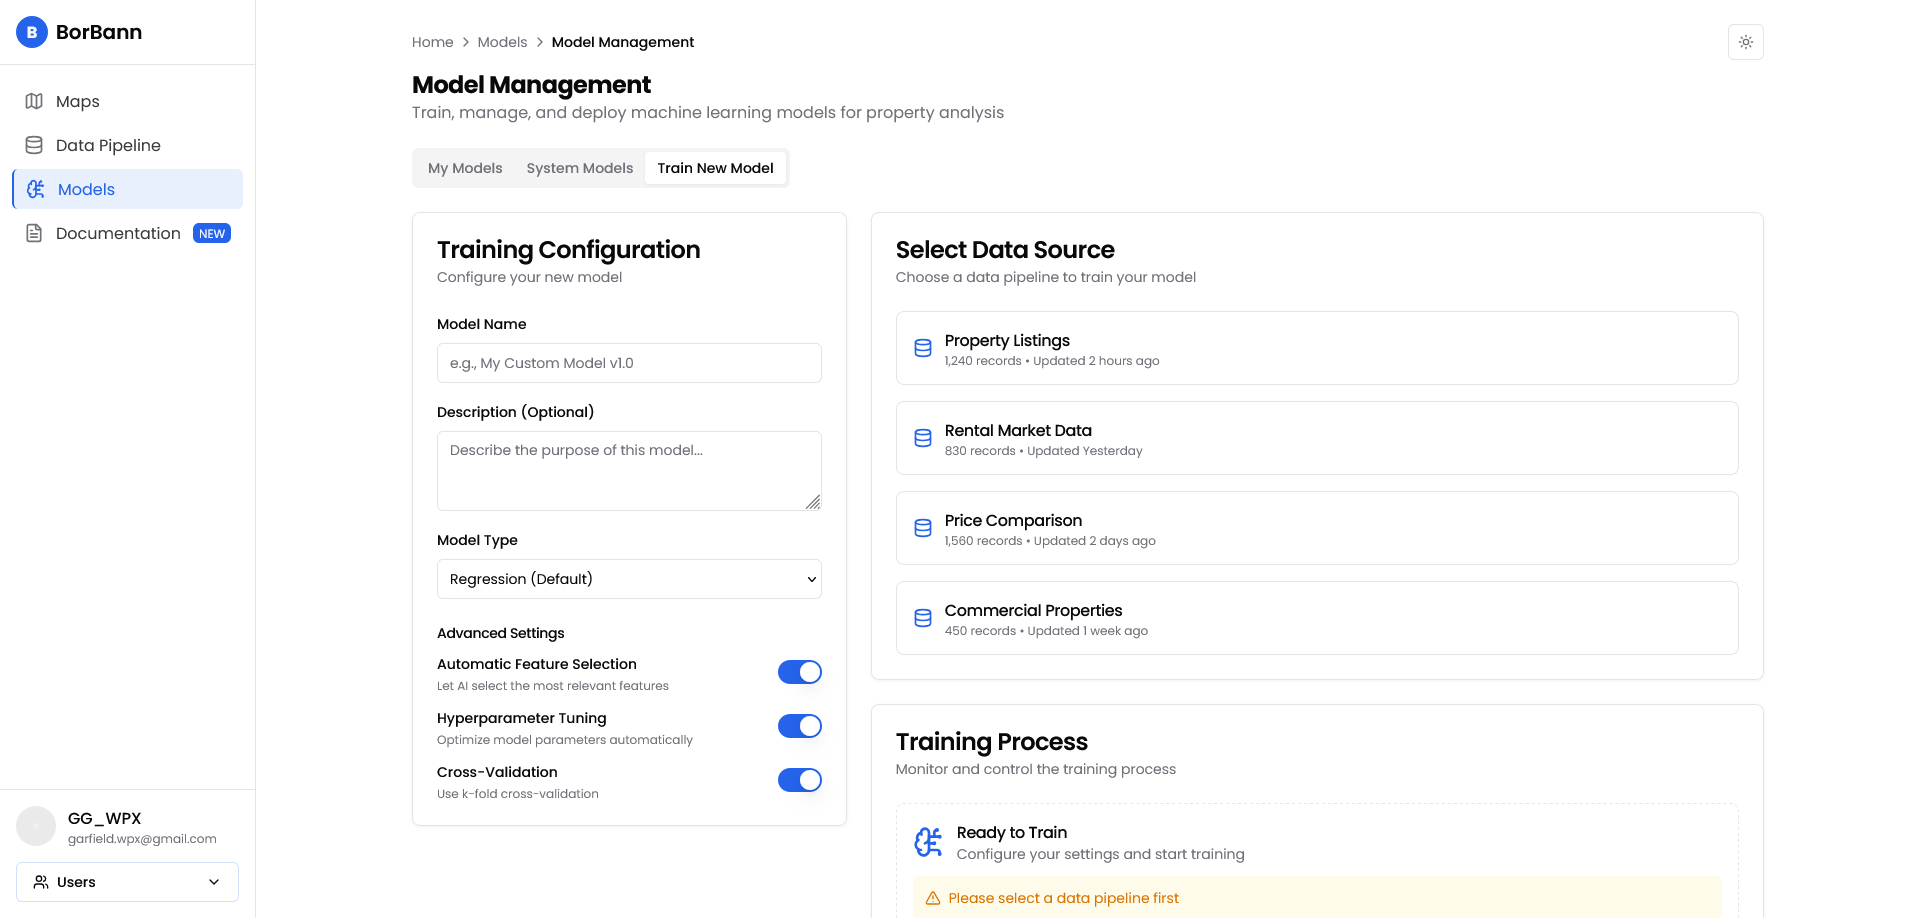
\includegraphics[width=1\textwidth]{assets/ui/models-new-model.png}
\caption{Model Creation Interface}
\label{fig:models-new-model}
\end{figure}

Figure \ref{fig:models-new-model} shows the model creation interface for configuring new prediction models. Users can select data pipelines as training sources and choose from recommended algorithms with explanations of their strengths.

\begin{figure}[h]
\centering
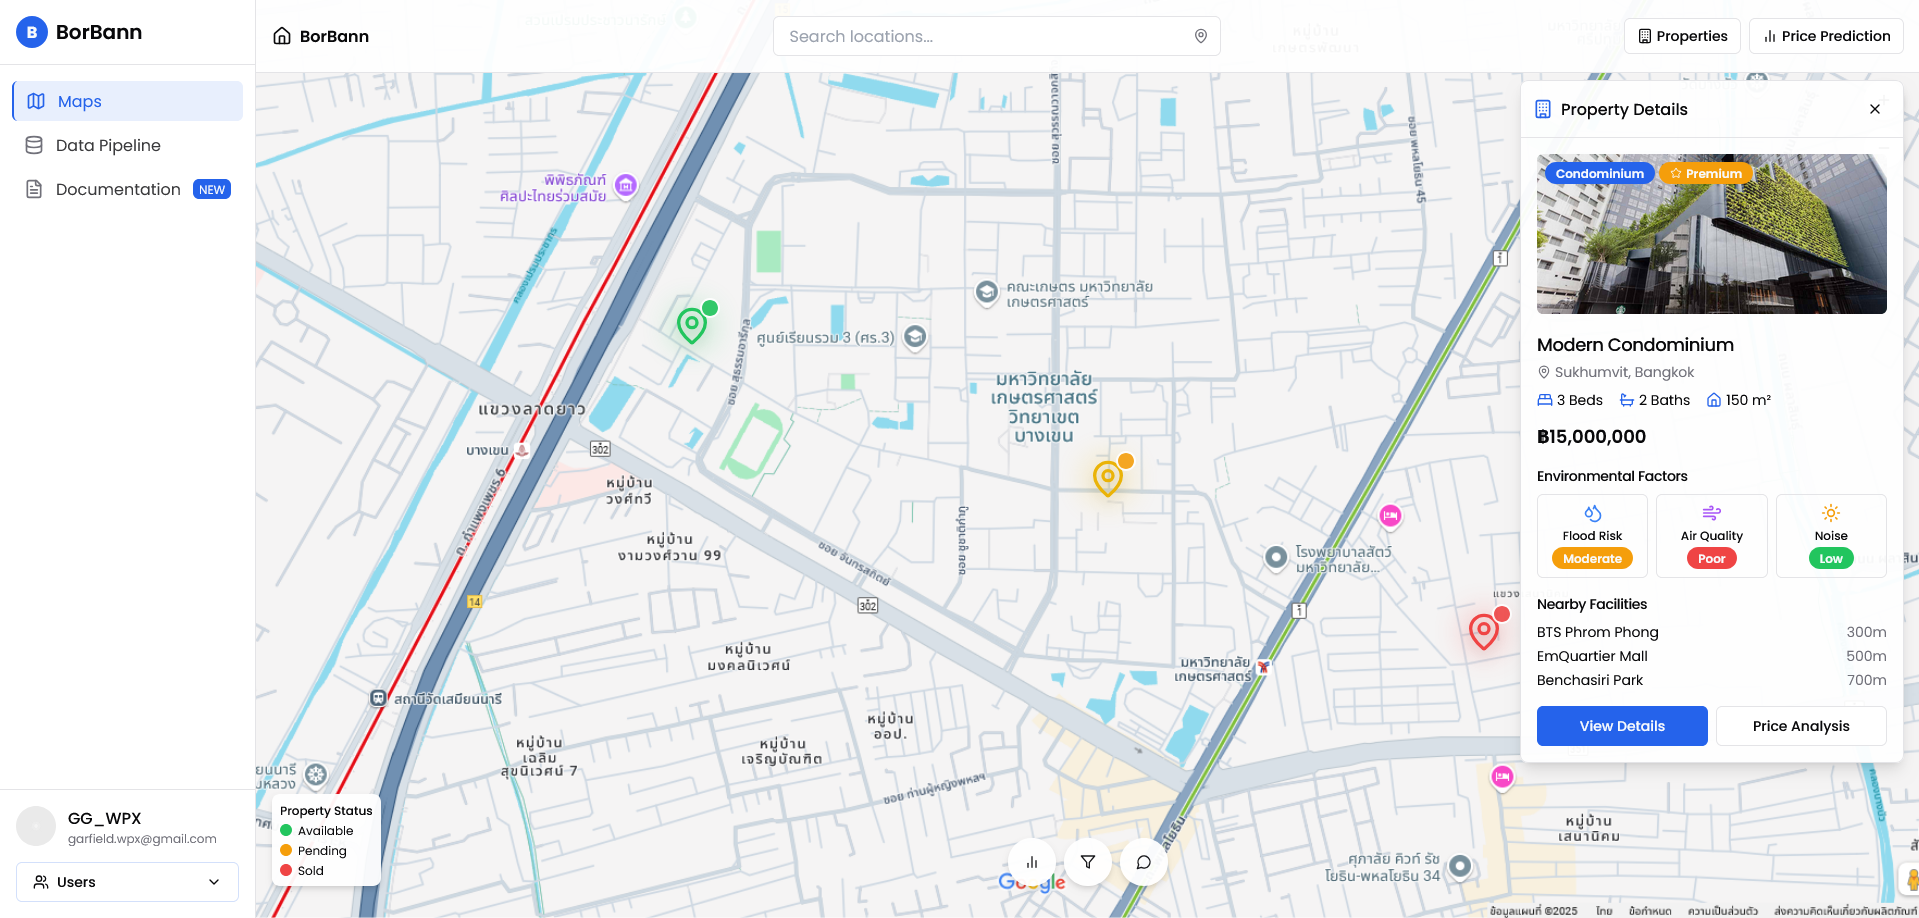
\includegraphics[width=1\textwidth]{assets/ui/map-page-main.png}
\caption{Geospatial Visualization - Main Map Interface}
\label{fig:map-page-main}
\end{figure}

Figure \ref{fig:map-page-main} displays the interactive property map with color-coded markers and navigation controls. The interface supports pan/zoom gestures and provides filtering options through the sidebar.

\begin{figure}[h]
\centering
\begin{minipage}[b]{0.45\textwidth}
\centering
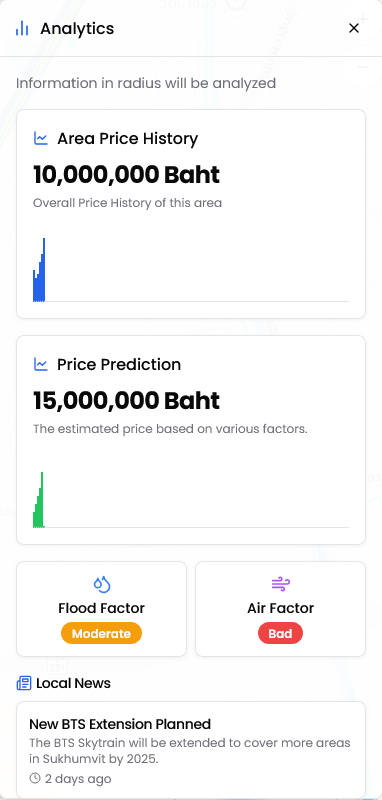
\includegraphics[width=\textwidth]{assets/ui/map-page-analytic.png}
\caption{Map Analytics Overlay}
\label{fig:map-page-analytic}
\end{minipage} \hspace{0.05\textwidth}
\begin{minipage}[b]{0.45\textwidth}
\centering
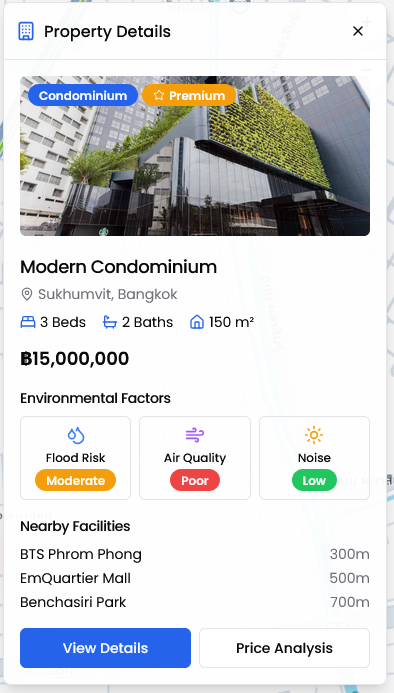
\includegraphics[width=\textwidth]{assets/ui/map-page-property-detail.png}
\caption{Property Detail Overlay}
\label{fig:map-page-property-detail}
\end{minipage}
\end{figure}

\pagebreak
Figure \ref{fig:map-page-analytic} shows environmental factor visualization through heat maps and data layers. This overlay helps users analyze contextual factors like pollution levels directly on the map.

Figure \ref{fig:map-page-property-detail} displays the popup that appears when users click map markers. This overlay provides immediate property information without requiring navigation away from the map.

\begin{figure}[h]
\centering
\begin{minipage}[b]{0.45\textwidth}
\centering
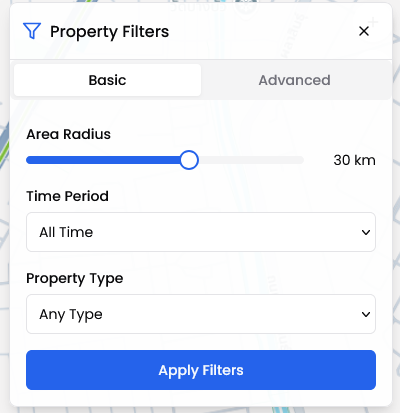
\includegraphics[width=\textwidth]{assets/ui/map-page-property-filter.png}
\caption{Property Filter Panel}
\label{fig:map-page-property-filter}
\end{minipage}
\hspace{0.05\textwidth}
\begin{minipage}[b]{0.45\textwidth}
\centering
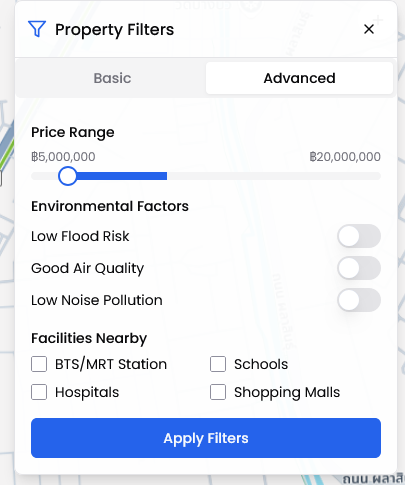
\includegraphics[width=\textwidth]{assets/ui/map-page-property-filter-advance.png}
\caption{Advanced Property Filter Options}
\label{fig:map-page-property-filter-advance}
\end{minipage}
\end{figure}

\pagebreak
Figure \ref{fig:map-page-property-filter} shows basic property filtering controls for price range, type and size parameters. The panel uses sliders and checkboxes for intuitive refinement of map results.

Figure \ref{fig:map-page-property-filter-advance} displays extended filtering options for specific amenities and neighborhood characteristics. These advanced parameters enable precise property matching based on detailed criteria.

\begin{figure}[h]
\centering
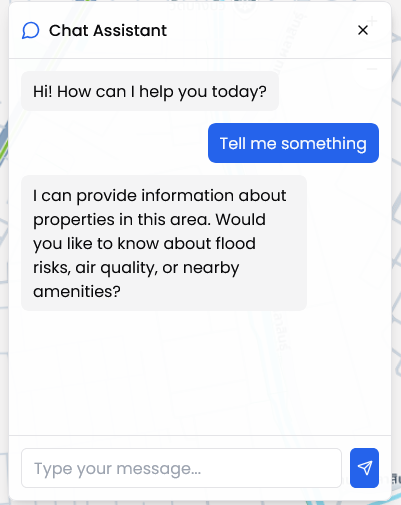
\includegraphics[height=0.5\textwidth]{assets/ui/map-page-chatbot.png}
\caption{Interactive Chatbot Assistant}
\label{fig:map-page-chatbot}
\end{figure}

Figure \ref{fig:map-page-chatbot} shows the conversational assistant for property search and analysis. The chatbot handles natural language queries about properties and market conditions.

\begin{figure}[h]
\centering
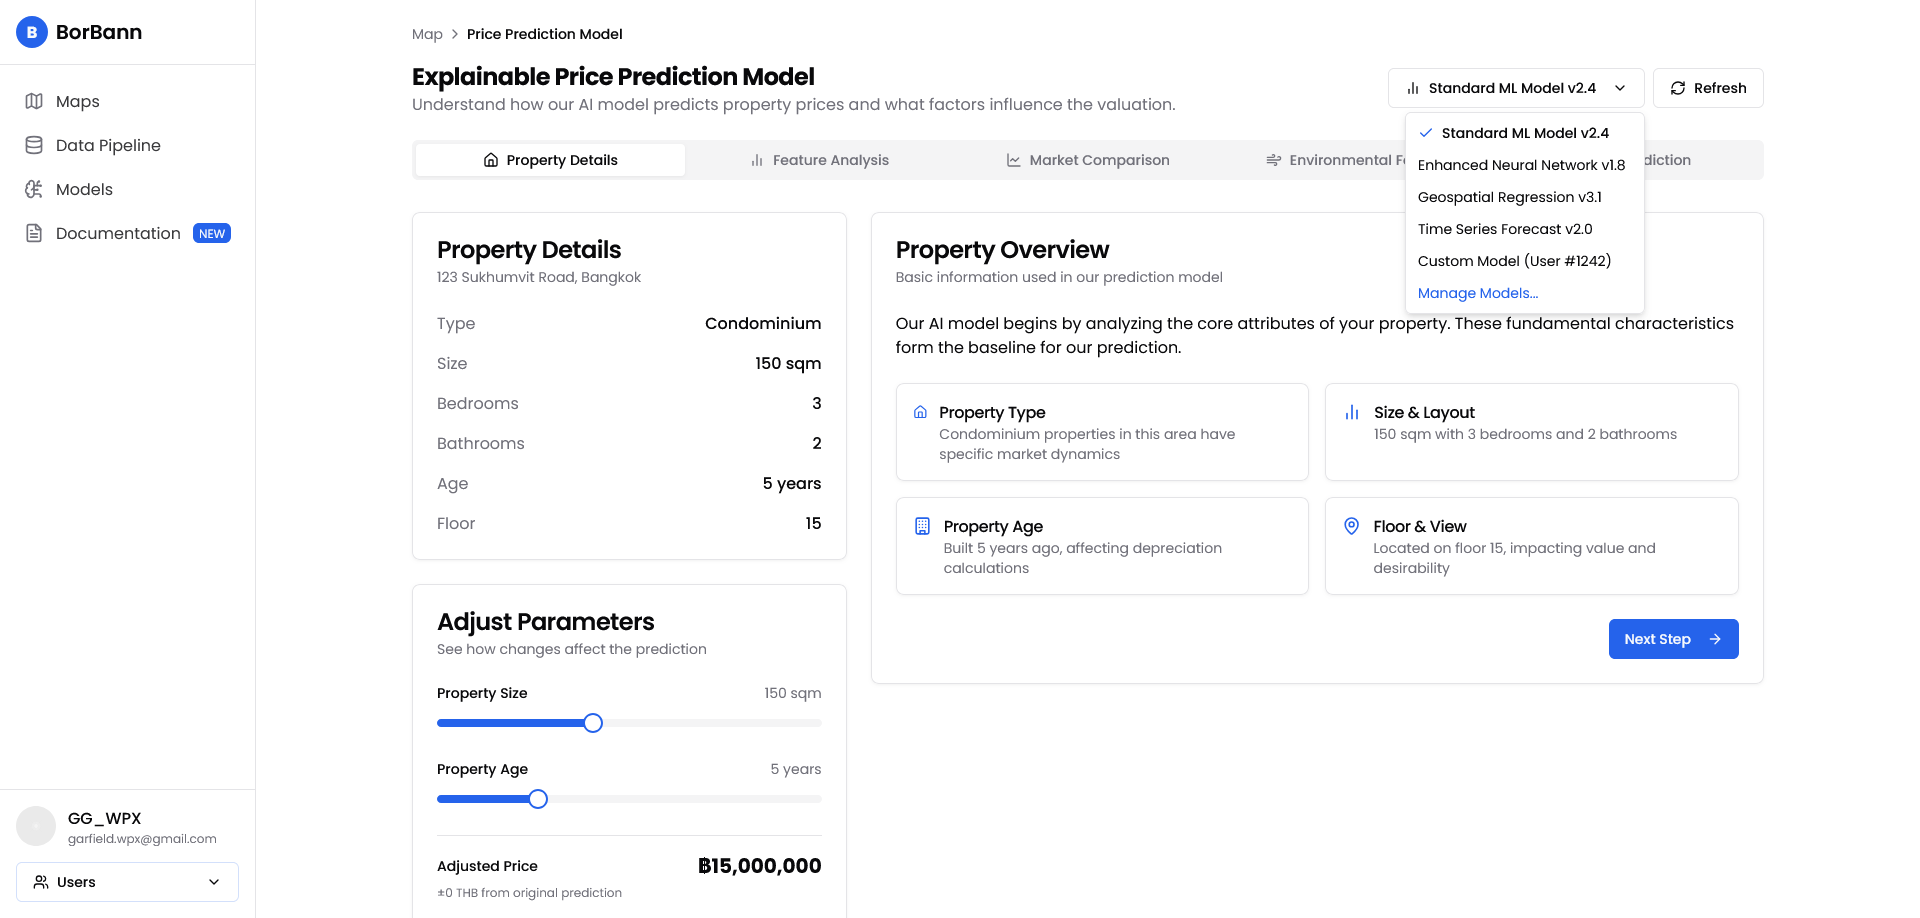
\includegraphics[width=1\textwidth]{assets/ui/explainable-property-detail.png}
\caption{Explainable Price Prediction - Property Overview}
\label{fig:explainable-property-detail}
\end{figure}

Figure \ref{fig:explainable-property-detail} displays the initial analysis of property attributes in the prediction model. The interface includes interactive parameter sliders that show how changes to property characteristics affect the predicted price.

\begin{figure}[h]
\centering
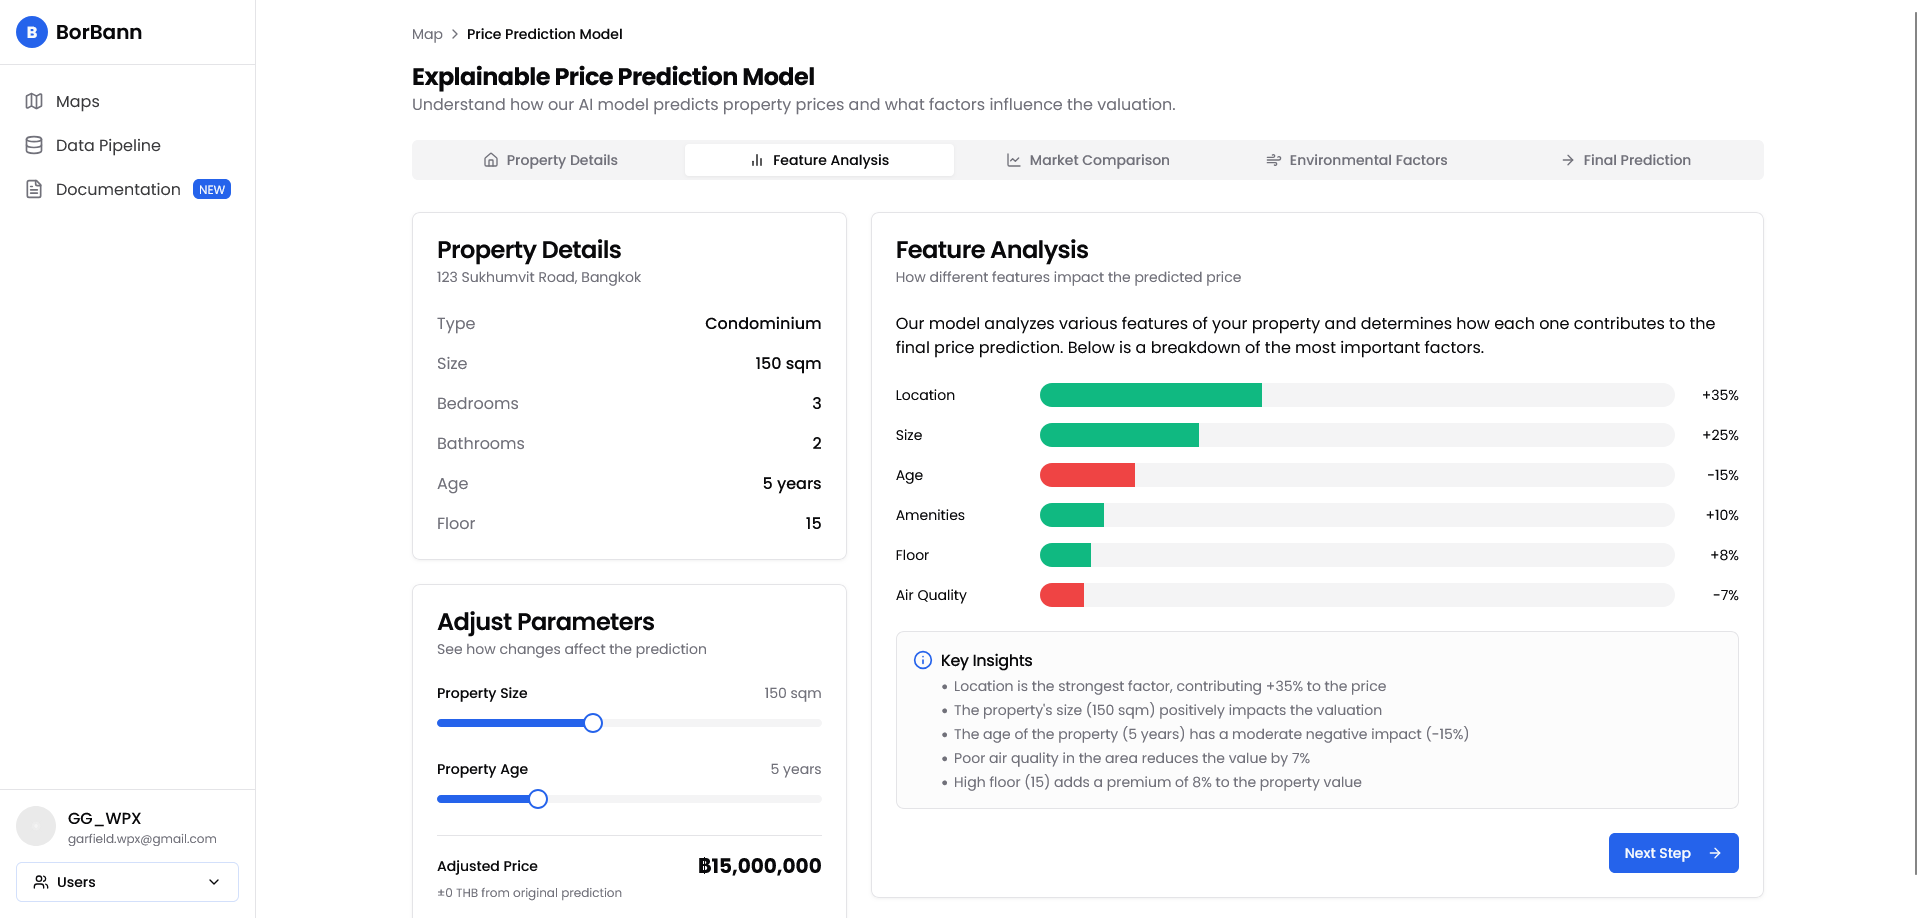
\includegraphics[width=1\textwidth]{assets/ui/explainable-feature-analysis.png}
\caption{Explainable Price Prediction - Feature Importance Visualization}
\label{fig:explainable-feature-analysis}
\end{figure}

Figure \ref{fig:explainable-feature-analysis} shows the contribution of different property features to the predicted price. The visualization uses color-coded bars to differentiate positive and negative factors with percentage impact values.

\begin{figure}[h]
\centering
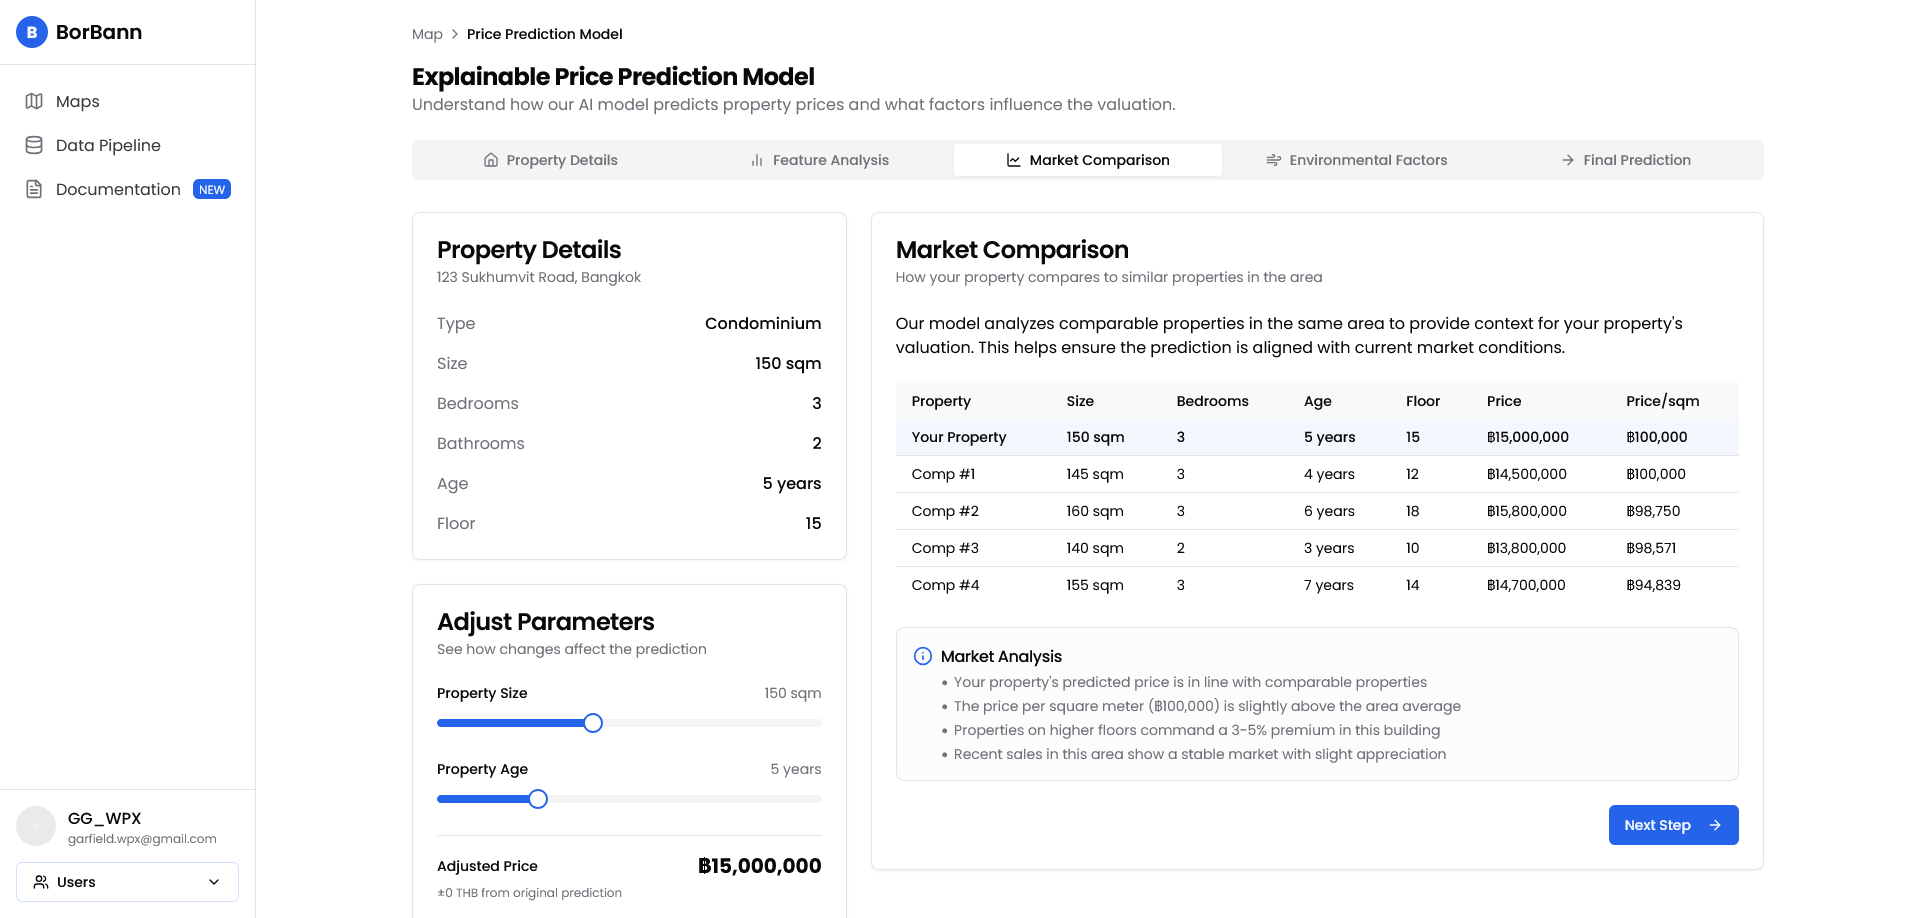
\includegraphics[width=1\textwidth]{assets/ui/explainable-market-comparison.png}
\caption{Explainable Price Prediction - Comparative Market Analysis}
\label{fig:explainable-market-comparison}
\end{figure}

Figure \ref{fig:explainable-market-comparison} presents a comparison of the subject property against similar properties in the area. The table highlights key attributes and pricing metrics with supporting analysis of market positioning.

\begin{figure}[h]
\centering
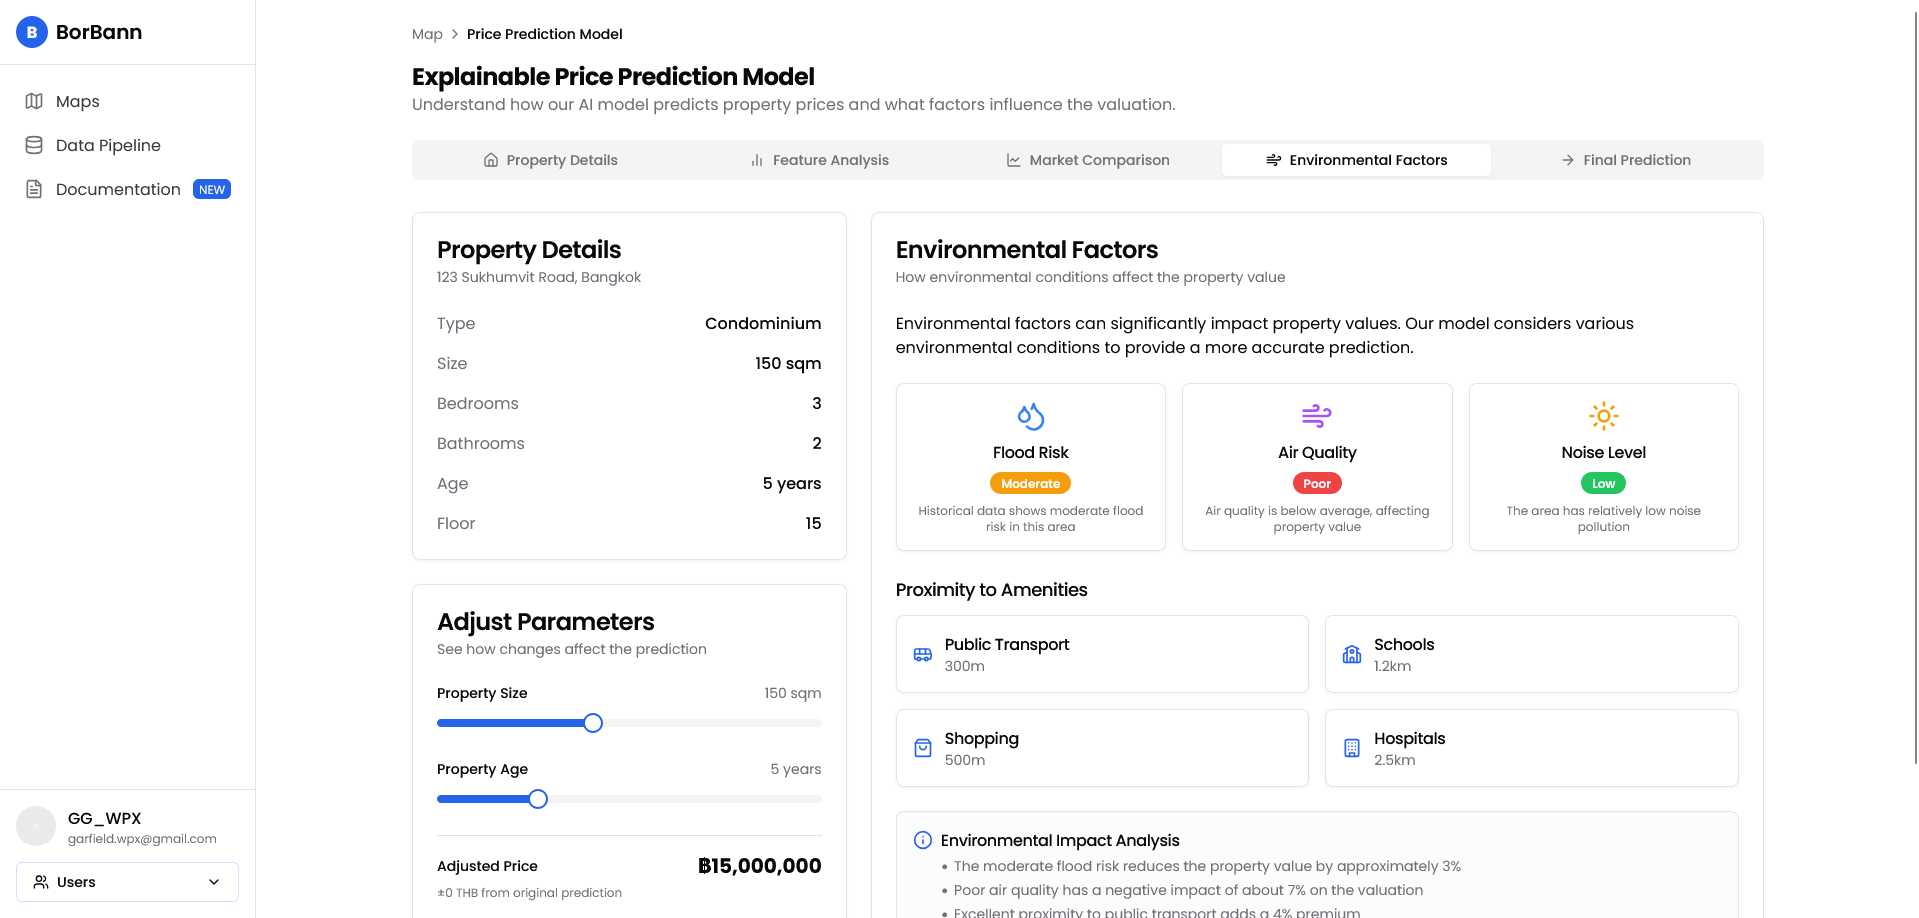
\includegraphics[width=1\textwidth]{assets/ui/explainable-environmental-factors.png}
\caption{Explainable Price Prediction - Environmental Impact Analysis}
\label{fig:explainable-environmental-factors}
\end{figure}

Figure \ref{fig:explainable-environmental-factors} analyzes environmental conditions and nearby amenities affecting property value. The interface displays flood risk, air quality, and proximity to key facilities with quantified impact on valuation.

\pagebreak
\begin{figure}[h]
\centering
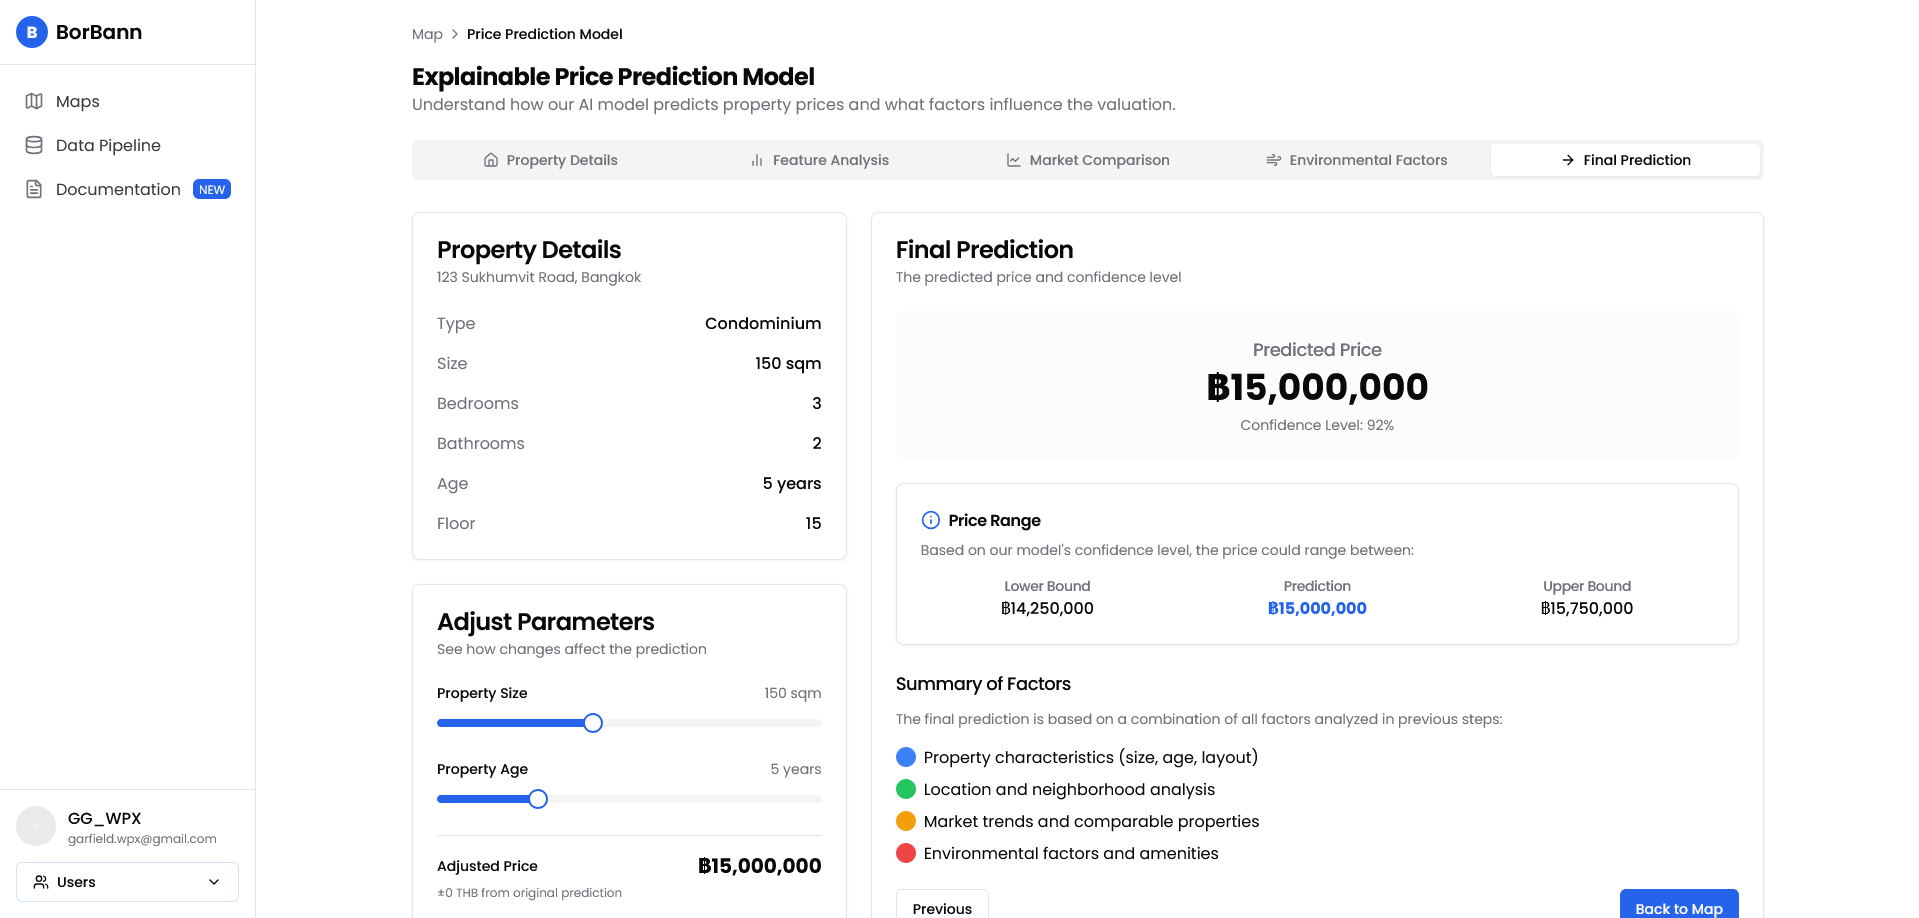
\includegraphics[width=1\textwidth]{assets/ui/explainable-final-prediction.png}
\caption{Explainable Price Prediction - Final Valuation with Confidence Range}
\label{fig:explainable-final-prediction}
\end{figure}

Figure \ref{fig:explainable-final-prediction} shows the final price prediction with confidence metrics and range indicators. The summary section explains how the valuation synthesizes insights from all analytical components.

\begin{figure}[h]
\centering
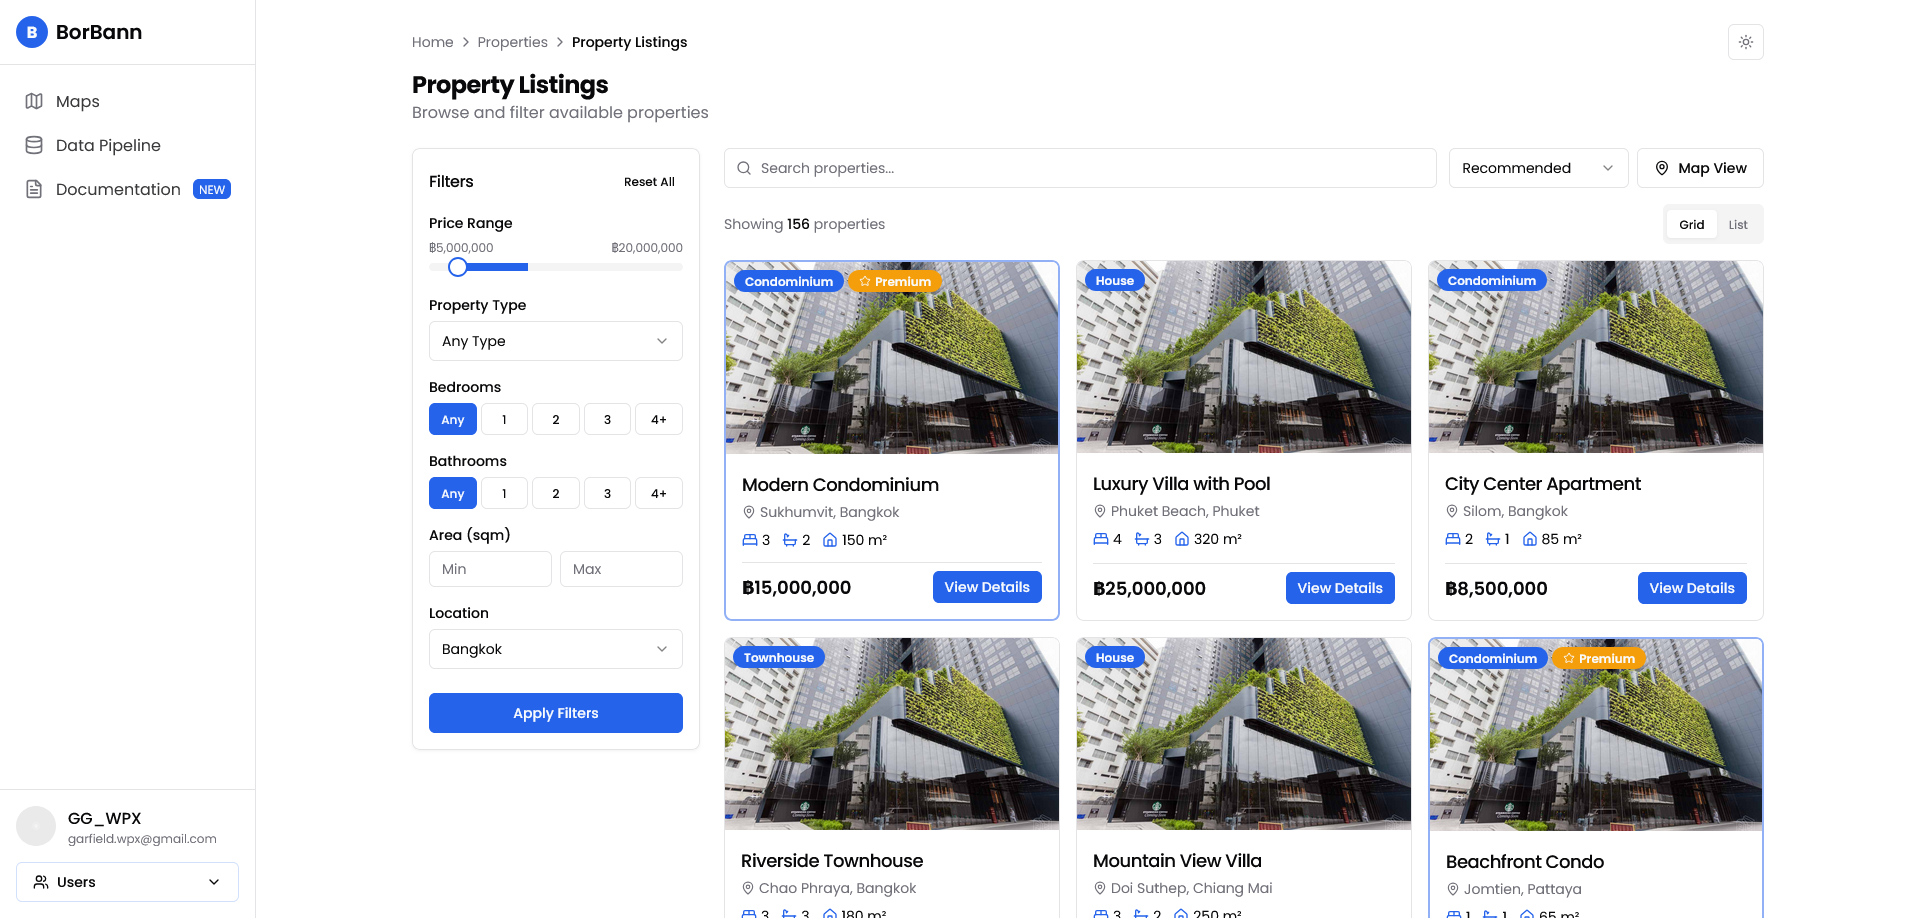
\includegraphics[width=1\textwidth]{assets/ui/property-listing-main.png}
\caption{Property Listings Page}
\label{fig:property-listing-main}
\end{figure}

Figure \ref{fig:property-listing-main} display property listings page with all listing that follow the filter tab the right.

\pagebreak
\begin{figure}[h]
\centering
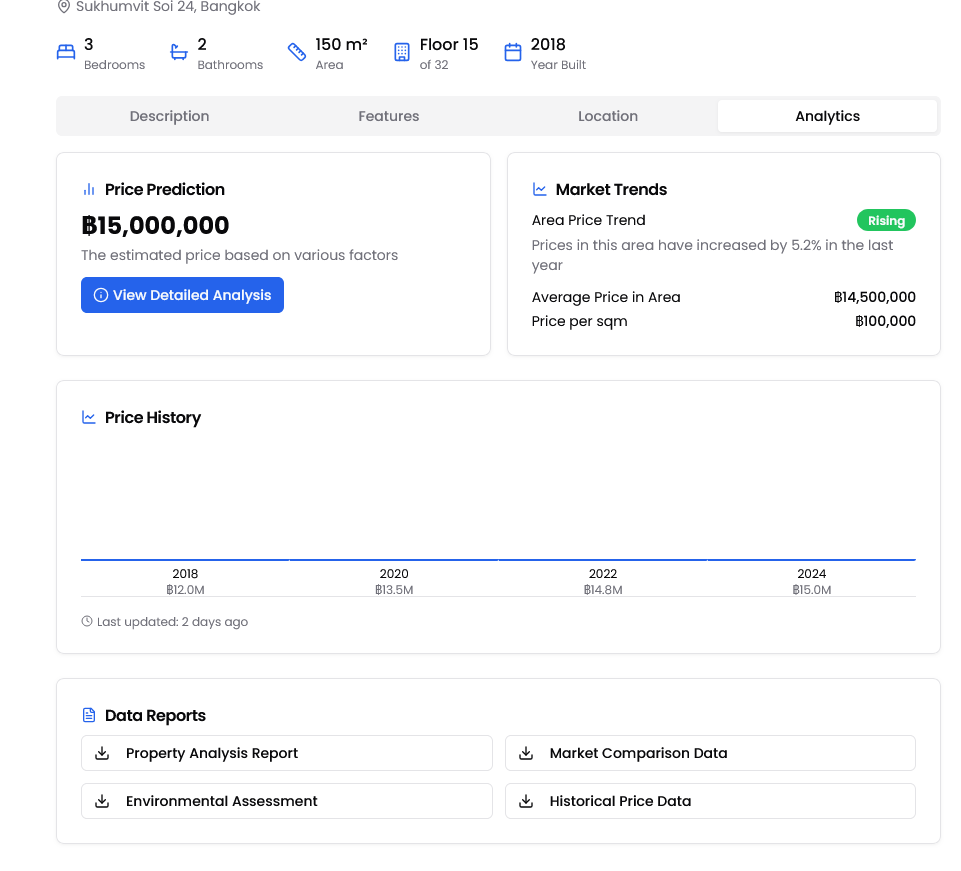
\includegraphics[width=1\textwidth]{assets/ui/property-listing-analytics.png}
\caption{Property Listings Page - Analytic Tab}
\label{fig:property-listing-analytics}
\end{figure}


Figure \ref{fig:property-listing-analytics} shows the analytic tab that show local context analytic of that specific listing.